
%
%%%%%%%%%%%%%%%%%%%%%
% Special Instructions
%%%%%%%%%%%%%%%%%%%%%
%
% Please follow these instructions to use line numbering package (lineno.sty):
%
%   http://fourforces.wordpress.com/2008/04/24/add-line-numbers-using-linenosty-in-revtex-4/
%

\RequirePackage{lineno}

\documentclass[aps,prc,twocolumn,groupedaddress,showpacs,amsmath,amssymb,floatfix,superscriptaddress]{revtex4}
\usepackage{multirow}
\usepackage{graphicx,subfigure}
\usepackage{times}
\usepackage{textcomp}
\usepackage{hyperref}

\bibliographystyle{apsrev}


\usepackage{color}

\newcommand{\nuebar}{$\overline{\nu}_{e}$}
\newcommand{\PerTonDay}{(ton$\cdot$day)$^{-1}$}
\hyphenation{KamLAND}

\begin{document}

\bibliographystyle{h-physrev3}

\title{Measuring Directionality in Double Beta Decay and Neutrino Interactions with Kiloton-Scale Scintillation Detectors}

% All university affiliations addresses go here:
\newcommand{\ucla}{\affiliation{University of California Los Angeles, Los Angeles, CA 90095, USA}}
\newcommand{\chicago}{\affiliation{University of Chicago, Chicago, IL, 60637, USA}}

%
\author{C.~Aberle}\ucla
\author{A.~Elagin}\chicago
\author{M.~Wetstein}\chicago
\author{H.~J.~Frisch}\chicago
\author{L.~Winslow}\ucla

\date{\today}

\begin{abstract}
Large liquid-scintillator-based detectors have proven to be
exceptionally effective for low energy neutrino measurements due to
their good energy resolution and scalability to large volumes. The
addition of directional information using Cherenkov light and fast
timing would greatly enhance the scientific reach of these detectors,
especially for searches for neutrinoless double-beta decay. In this
paper, we develop a technique for extracting particle direction and
evaluate different detector advances that could be used to make
direction reconstruction a reality in a kiloton-scale detector.
\end{abstract}

\pacs{23.40.$-$s, 21.10.Tg, 14.60.Pq, 27.60.$+$j}

\maketitle

\section{Introduction}
Liquid scintillator based detectors are responsible for several of the
critical measurements that have determined our present understanding
of neutrino masses and mixings. These measurements include KamLAND's
measurement of reactor antineutrino oscillation at a distance of
$\sim$200~km\cite{kam2013}, Borexino's measurement of $^{7}$Be solar
neutrino oscillation\cite{borexino}, and most recently the short
baseline reactor antineutrino experiments that measured oscillations
due to $\theta_{13}$ at a distance of 1~km: Daya Bay\cite{dbtwo},
Double Chooz\cite{dctwo, dchydrogen}, and RENO\cite{reno}.
Scintillator-based neutrino detectors will continue to be important for the
next set of neutrino measurements, from the determination of the
neutrino mass hierarchy\cite{juno,reno50} to elastic scattering
measurements\cite{isodarscatt} and sterile neutrino
searches\cite{isodar,nist} and for non-proliferation
applications\cite{nucifer, songs}.

The scalability of these detectors to large volumes also makes them
highly competitive for neutrinoless double-beta ($0\nu\beta\beta$)
decay searches in which the final state consists of a
positron-electron pair with energies in the few MeV range.  Currently
one of the best limits for the $0\nu\beta\beta$ half-life comes from
KamLAND-Zen\cite{KZ0nu}.

The advantage of liquid scintillators for measurements in the
$\sim$1~MeV range is their scalability from 1~ton to 1~kiloton while
providing energy resolutions of $\sim$5\%. This is roughly a factor of
two better than water Cerenkov detectors, the other developed
technology that can be economically scaled to these large
masses. However, for scintillator-based detectors, while the energy
resolution is good due to the abundance of light, the light is
isotropic and does not retain the directional information of the
primary particle.  In contrast, the direction of the particle can be
reconstructed from the Cerenkov cones in water-based detectors,
although the energy resolution rapidly degrades below $\sim$5~MeV. For
double-beta decay in particular, but also for neutrino interactions,
the directional information can be a strong suppressant of
backgrounds.

In a liquid-scintillation-based detector, Cerenkov light is also
produced, although most is absorbed and re-emitted as part of the
scintillation processes.  However, some fraction retains its
directional information. If this directional Cerenkov light can be
isolated from the copious isotropic scintillation light, it may be
possible to reconstruct the direction of the primary particle or, in
the case of double beta decay, to determine the existence and topology
of the pair.  The addition of directionality is thus a powerful tool
for background rejection.  In this paper, we develop a technique for
separating the Cerenkov and scintillation using the photon arrival
times and evaluate different detector technologies that would allow
the realization direction reconstruction in kilo-ton scale
scintillating neutrino detectors.

\section{Light Production in Liquid Scintillators}
Liquid scintillators are cocktails of aromatic hydrocarbons. When
charged particles move through a scintillator, the molecules are
excited, predominantly the the non-localized electrons in the
$\pi$-bonds of the phenyl groups~\cite{scintillator_ref}. Vibrational
and rotational modes of the molecules are turned into heat within
picoseconds through collisions with other molecules.  Within $\sim$10
picoseconds, the $\pi$-electrons de-excite to the first excited state
from higher levels through radiationless transitions. The first
excited state de-excites through photon emission. There are two
characteristic times for this de-excitation, depending if the singlet
state or the triplet state was excited.  The singlet state will
de-excite within nanoseconds while the triplet state de-excites on the
order of 10's or 100's of nanoseconds. These two processes are
fluorescence and phosphorescence respectively. The exact time
constants for these processes are determined by the composition of the
scintillator.

The molecules in liquid scintillators are not isolated. Radiationless
processes transfer energy between the molecules. The probability of
energy transfer between molecules increases as the overlap between the
molecule's absorption and emission spectra increase. The absorption
and emission spectra overlap at some level for all
molecules. Consequently if there is only one type of molecule in the
scintillator cocktail, the light output would be reduced due to
inefficiencies in the energy transfer through multiple absorption and
reemission processes. Aromatic solutes or fluors are added to the
primary solvent to shift the wavelength of the photons to longer
wavelengths where the scintillator is more transparent. This
wavelength-shifting is also used to match the quantum efficiency as a
function of wavelength for the photodetectors being used. One typical
scintillator mixture uses pseudo-cumene as the solvent with 1-5~g/L of
PPO as the fluor. This mixture has a peak emission at about 400~nm
where bialkali photomultiplier tubes (PMTs) are most sensitive and the
pseudo-cumene is relatively transparent.

A good liquid scintillator will produce $\sim$10,000 photons
isotropically per MeV of deposited energy. Although less abundant,
Cerenkov light will be produced as well if a particle is moving faster
than the speed of light in the medium.  This light is emitted in a
cone pointed in the direction of the particles trajectory and with a
continuous spectrum weighted toward shorter wavelengths
but extending well into the red. The spectrum is described by:
\begin{equation}
\label{eqCerenkov}
\frac{dN}{d\lambda dx} = \frac{2 \pi \alpha Z^2}{\lambda^2} ( 1 - \frac{1}{\beta^2 n(\lambda)^2} )
\end{equation}
where $n(\lambda)$ is the wavelength-dependent index of refraction and
$\beta$ is the velocity of the incoming particle. The Cerenkov light
produced at wavelengths shorter than the absorption cutoff of the
scintillator will be absorbed and re-emitted as isotropic light, but
wavelengths longer than this cutoff will propagate across the
detector, retaining their directional information. The yield is
roughly 60 photons per MeV, assuming a 400~nm absorption
cutoff\cite{qdot}. These undisturbed Cerenkov photons will have timing
determined by the group velocity \cite{group_velocity_article} in the liquid,
\begin{equation}
\label{eqGroup}
v_{g}(\lambda) = \frac{c_{vacuum}}{n(\lambda) + dn(\lambda)/dlog(\lambda)}.
\end{equation}
In Geant4 optical photons are assigned the group velocity in the wavelength 
region of normal dispersion ($dn(\lambda)/dlog(\lambda)$>0) which is relevant to 
our study. 
The longer wavelengths Cerenkov photons typically arrive before
the scintillation light, which is slowed by both the scintillation
processes and the shorter wavelengths involved. Thus, with sufficient
timing resolution and sensitivity to longer wavelength, it should be
possible to separate the directional Cerenkov light and the isotropic
scintillation light in time and then reconstruct the direction of the
initial particle.

\section{Geant4 Simulation}
In order to study the effects relevant to directionality reconstruction in liquid scintillators, a Geant4 \cite{geant4one,geant4two} simulation has been set up. The presented simulation application has been developed using standard Geant4 functionality for the optical model of the liquid scintillator. Version Geant4.9.6 is used and the simulation application has been built from a customized official application example. The simulation is kept simple to provide generally applicable information about the main factors in directionality reconstruction. 

The implemented detector geometry is a sphere of 6.5~m (or 0.65~m) diameter filled with liquid scintillator. Default scintillator properties have been chosen to match the KamLAND scintillator \cite{tbd}: 80~\% n-Dodecane, 20~\% Pseudocumene (1,2,4-Trimethylbenzene) and 1.52~g/l PPO (2,5-Diphenyloxazole). The implemented scintillator properties include the atomic composition and density ($\rho$ = 0.7752~g/ml), the wavelength-dependent attenuation length and refractive index, the scintillation emission spectrum, emission rise time ($\tau_r$ = 1.0~ns) and emission decay time constants ($\tau_{d1}$ = 6.9~ns and $\tau_{d2}$ = 8.8~ns with relative weights of 0.87 and 0.13), scintillator light yield (LY, 9030.5 photons/MeV) and the Birks constant ($kB$ = 0.106~mm/MeV) \cite{tbd}. Variations from the baseline KamLAND case are discussed below when applicable. Reemission of absorbed photons in the scintillator bulk volume and scattering has not been included. Reflections, reemission and scattering are expected to be corrections to the main effects studied in this paper and are subject of future work. 

The sphere surface is used as the photodetector. It is treated as fully absorbing (no reflections) with a coverage of 100~\%. Two important photodetector properties have also been varied: Transit time spread (TTS, default $\sigma$ = 0.1~ns) and wavelength-dependent quantum efficiency (QE) for photoelectron production. The default is the bialkali photocathode of the Double Chooz photomultiplier tubes (PMTs) \cite{tbd}. It has been verified to be the same type as the KamLAND photocathode. We used the Double Chooz QE because the data was available with finer spacing in wavelength.

%deprecated text: fake vertex reconstruction not needed anymore. 
%To this end, we use the KamLAND vertex resolution of 12.0~cm \cite{tbd} ($\sigma$ in one dimension) to randomly draw a vertex around the known true vertex for each event. This vertex is subsequently used as a reconstructed vertex and consequently, a time of flight (TOF) correction relative to the center of the sphere is applied for each photon hit depending on the distance between the reconstructed vertex and the hit position on the sphere. For the TOF correction a single effective speed of light is used. This effective speed was extracted at the mean wavelength of both Scintillation and Cerenkov photons (408~nm). The 12.0~cm vertex resolution corresponds to a time resolution broadening of about 0.6~ns ($\sigma$). Note that the vertex resolution itself is dependent on scintillator and detector properties. For example, the PMTs used in KamLAND have a TTS of 1.28~ns ($\sigma$) and significant improvement of the vertex resolution could be possible with faster photodetectors. In section \ref{reconstruction_sec}, we discuss first results on more realistic reconstruction.
\begin{figure*}[tbh]
        \begin{center}
        \subfigure[Default simulation.]{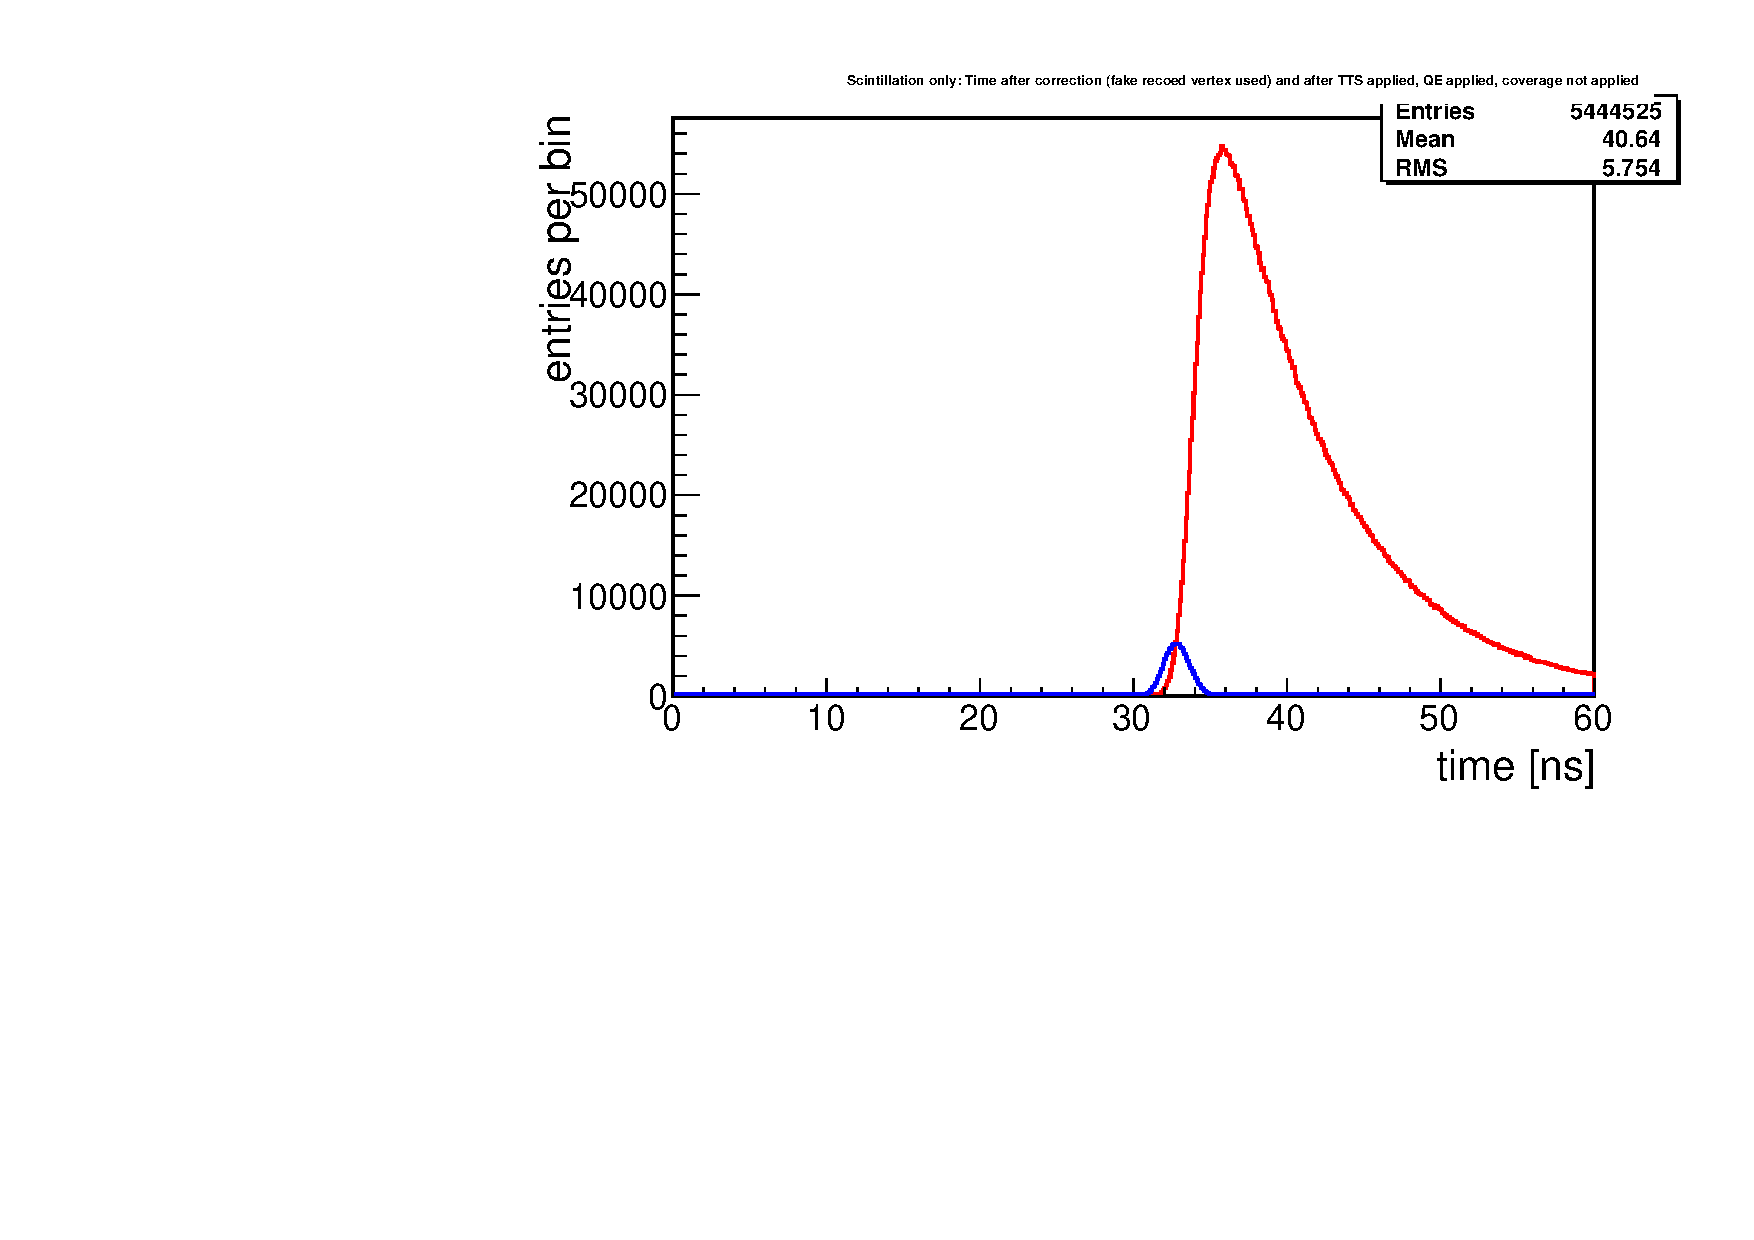
\includegraphics[scale=0.295]{graphs/6p5Meter_5MeVElectrons_Bialkali_KamlandScintSpec_TIME.pdf}}
        \subfigure[Increased TTS (1.28~ns).]{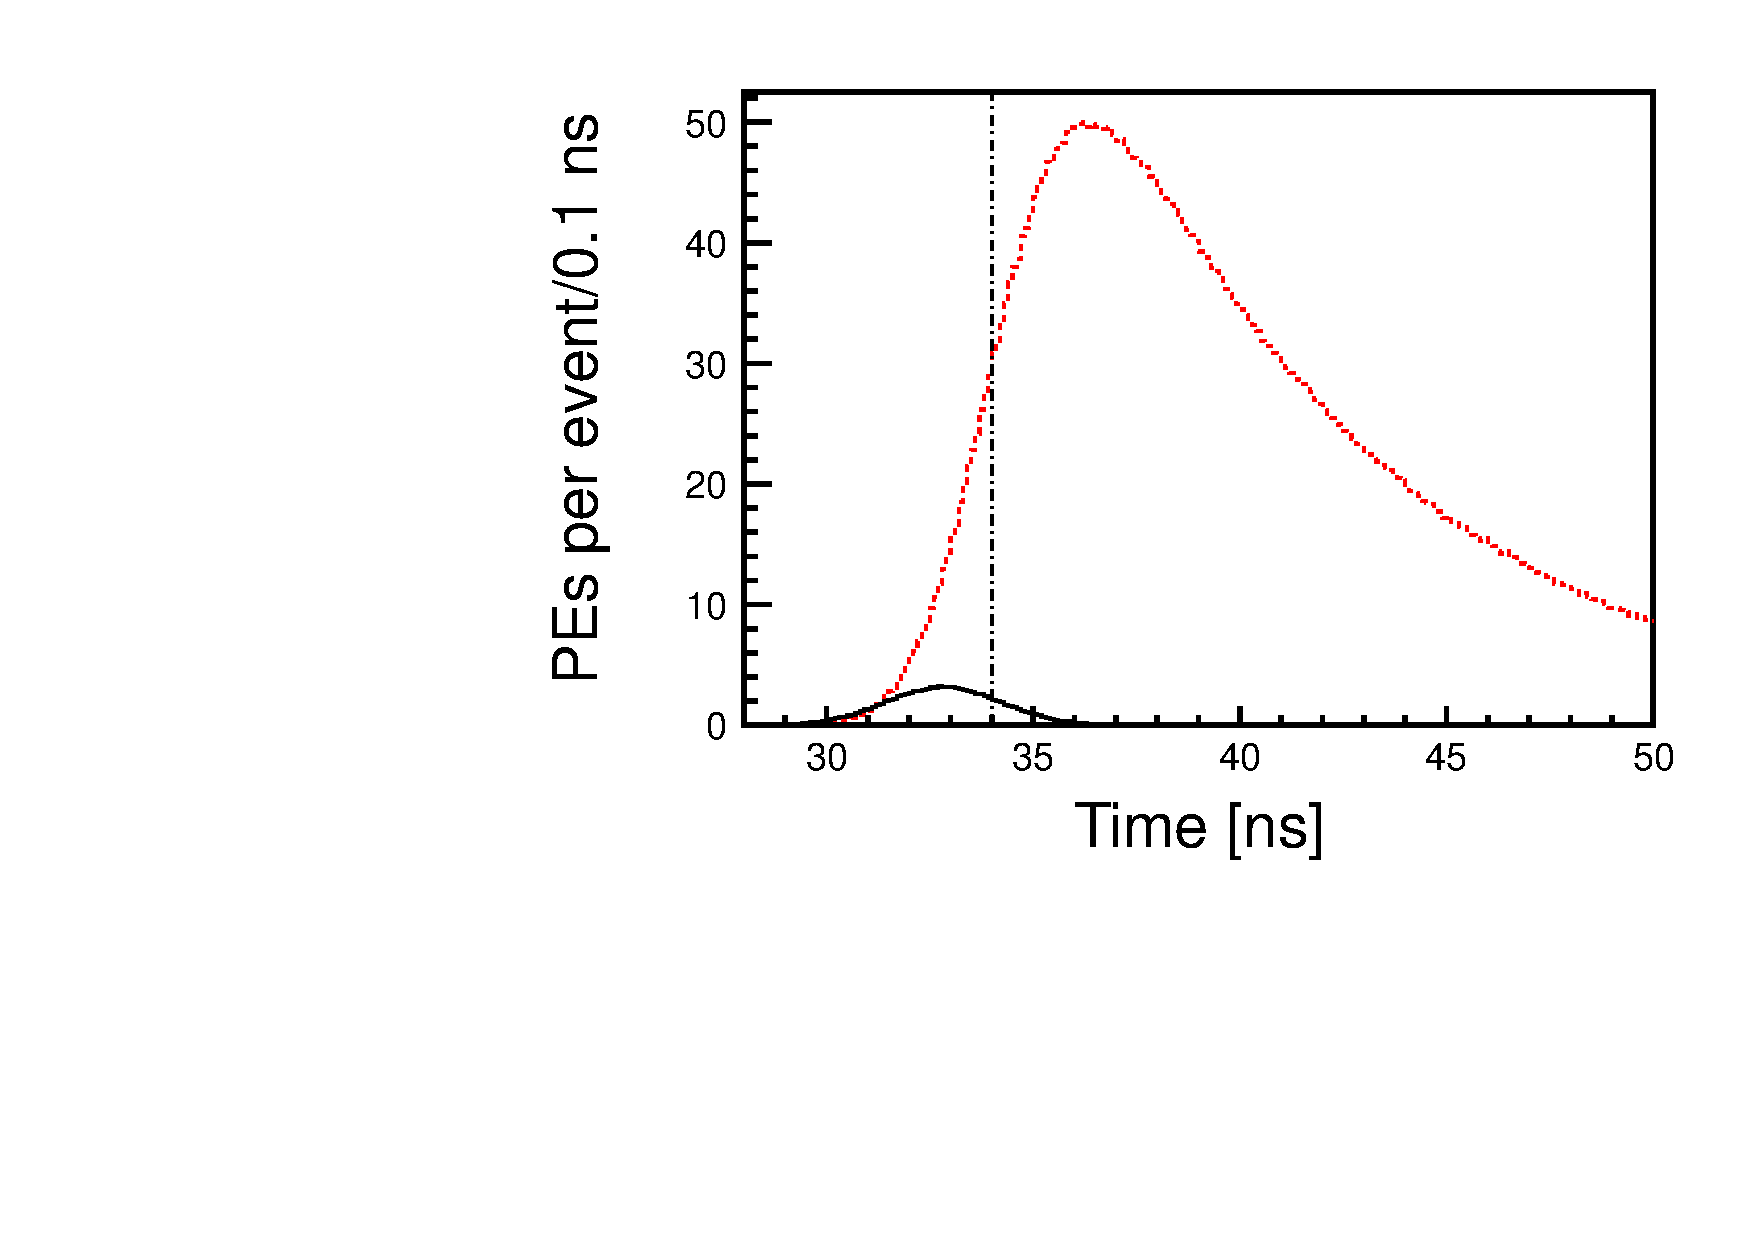
\includegraphics[scale=0.295]{graphs/6p5Meter_5MeVElectrons_Bialkali_KamlandScintSpec_1p28nsTTS_TIME.pdf}}
        \subfigure[Red-sensitive photocathode.]{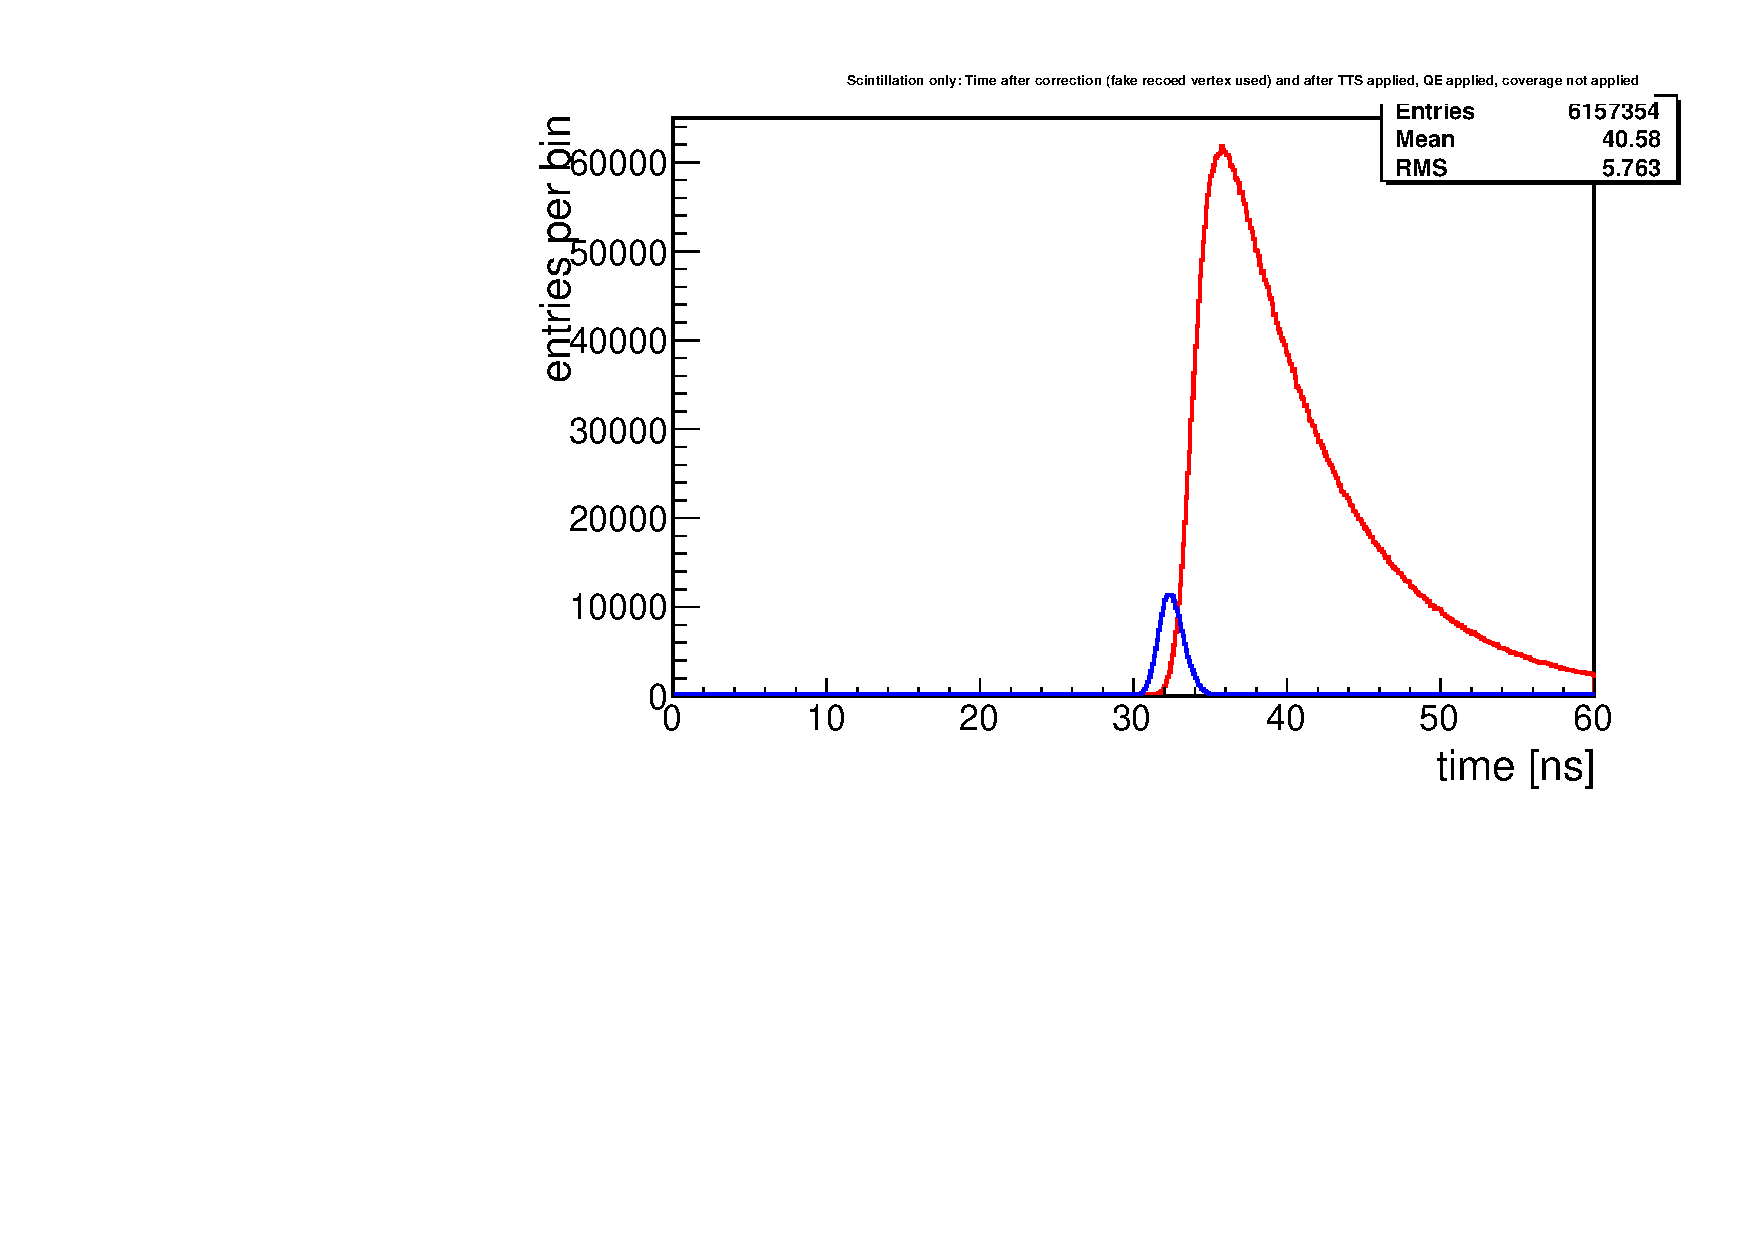
\includegraphics[scale=0.295]{graphs/6p5Meter_5MeVElectrons_RedSensitiveQE_KamlandScintSpec_TIME.pdf}}
        \caption[]{PE times after TTS application for the simulation of 1000 electrons (5~MeV) with different settings. PEs from Cerenkov light (black) and scintillation light (grey) are compared. The dashed vertical line illustrates a time cut at 34~ns. (a) Default simulation including bialkali photocathode and TTS = 0.1~ns ($\sigma$). The number of PEs per event after the 34.0~ns time cut is 171 from scintillation and 108 from Cerenkov. (b) Default simulation settings but for TTS = 1.28~ns (KamLAND 17 in. PMTs). The number of PEs per event after the 34.0~ns time cut is 349 from scintillation and 88 from Cerenkov. (c) Default simulation settings but for GaAsP photocathode. The number of PEs per event after the 34.0~ns time cut is 50.8 from scintillation and 171 from Cerenkov. \label{time_plots_comparison}}
        \end{center}
\end{figure*}
Before we discuss the simulation results for different simulation settings in the following sections, we highlight the effects which contribute to the timing of the scintillator detector system. First, the simulated travel time of the initial 5~MeV electron is between 0.10 and 0.15~ns, while the travel distance is about 3~cm. Second, the scintillation light emission follows a scintillator-specific distribution characterized by rise and decay time(s). Before the solutes in liquid scintillator can emit optical photons, the energy has to be transfered from the solvent to the solute. The time constant of this energy transfer accounts for a rise time in scintillation light emission. Past neutrino experiments were not highly interested in the effect of scintillation rise time which is the reason why there is a lack of accurate numbers. We assume a rise time of 1~ns, more detailed studies are needed in the future. The two time constants used to describe the falling edge of the scintillator emission time distribution (quoted above) are values specific to the KamLAND scintillator. Third, chromatic dispersion turns out to be an important effect in a 6.5~m diameter detector at the level of precision needed for direction reconstruction. Due to the wavelength-dependence of the refractive index the speed of light in the scintillator (the group velocity is used in Geant4 for normal dispersion) is also wavelength dependent. In order to study the size of this effect, we extracted results from a simplified simulation of 5~MeV electrons at the center of the sphere where we used instantaneous scintillation and did apply neither TTS nor TOF correction. The true time distributions of photoelectrons were analyzed for scintillation light and Cerenkov light separately. Photoelectrons coming from Cerenkov light are created about 0.5~ns earlier than PEs from scintillation light on average. The RMS values for both the Cerenkov and scintillation light true PE time distributions are both about 0.5~ns. Note that these numbers include the effect of the finite electron travel time.

On the detector side, the time information of single photoelectrons is affected by the TTS of the photodetectors, a number which can be different by orders of magnitude depending on the detector type. The default TTS of 0.1~ns ($\sigma$) is a value which can be achieved with the large area picosecond photodetectors (LAPPDs)\cite{LAPPDSum,LAPPDTDR} and possibly hybrid photodetectors (HPDs)\cite{hpdThesis}. In fact, even significantly lower TTS numbers are realistic with the LAPPD. Finally, the accuracy of the vertex reconstruction is reflected in broadening and distortions of the time spectrum (after the TOF correction has been applied). Another effect which is to be addressed in future work is the granularity of the photodetectors which adds to the uncertainty in the light path and thus the TOF correction.   

In Sections \ref{detector_timing_sec} to \ref{edep_size_sec}, we comparatively study the photoelectron timing for different detector properties. We follow the idea to increase discrimination between Cerenkov and scintillation light by detector timing. The main quantities provided by the Geant4 simulation are the photoelectron hit positions and the detection times after TTS has been applied. In section \ref{reconstruction_sec} these quantities are used for event reconstruction.
%%statement that rise time is not super-crucial (see April 11 talk)
%% include wavelength spectra, emission spectra, absorption (?), refractive index  ?
%% Other settings: physics list, theCerenkovProcess->SetMaxNumPhotonsPerStep(20);theCerenkovProcess->SetMaxBetaChangePerStep(10.0); theCerenkovProcess->SetTrackSecondariesFirst(true); theScintillationProcess->SetScintillationYieldFactor(1.); theScintillationProcess->SetTrackSecondariesFirst(true); theScintillationProcess->SetFiniteRiseTime(true); particle gun, 5MeV e- in x direction from center, random polarization
%% discussion: can chromatic dispersion be disentangled? With very high statistics maybe yes (see Ben Monreal, Matt Wetstein).
%% discussion: many scintillator properties depend on each other. Optimization of scintillator properties could lead to better results for directionality reconstruction. i.e. slower scintillation (but vertex reco worse!, LY tends to be lower) , lower wavelength, 
%% idea: filter for part of the PMTs or two kinds of PMTs: separation by wavelength
%% coverage is just a reduction by factor 0.22 (flat over wavelengths etc.), not studied in the paper?  
%% at the 0.1 ns level in a 6.5 m detector one has to be careful with the input of nref. If the slope is not smooth enough the group velocity calcuation is creating wavelength-dependent distortions. 
%% Reflections and absorption/reemission and scattering will shift events to higher times were they will likely not pass the time cut. They will effectively change the scintillation/Cerenkov ratio. Scattering might distort the angular variables and is subject of future work. 
%% In small det. the chromatic dispersion doesn't help too much. (In the small detector the detector properties are the driving factor.)
%% discussion: some scintillator and detector properties have complicated effects on the directionality, also other requirements have to be considered (high LY, high resolutionc). Multiparameter optimization problem.  
%% nuebar scattering --> one of next paper

\section{Detector Timing}
\label{detector_timing_sec}
%%\begin{figure}
%%        \begin{center}
%%        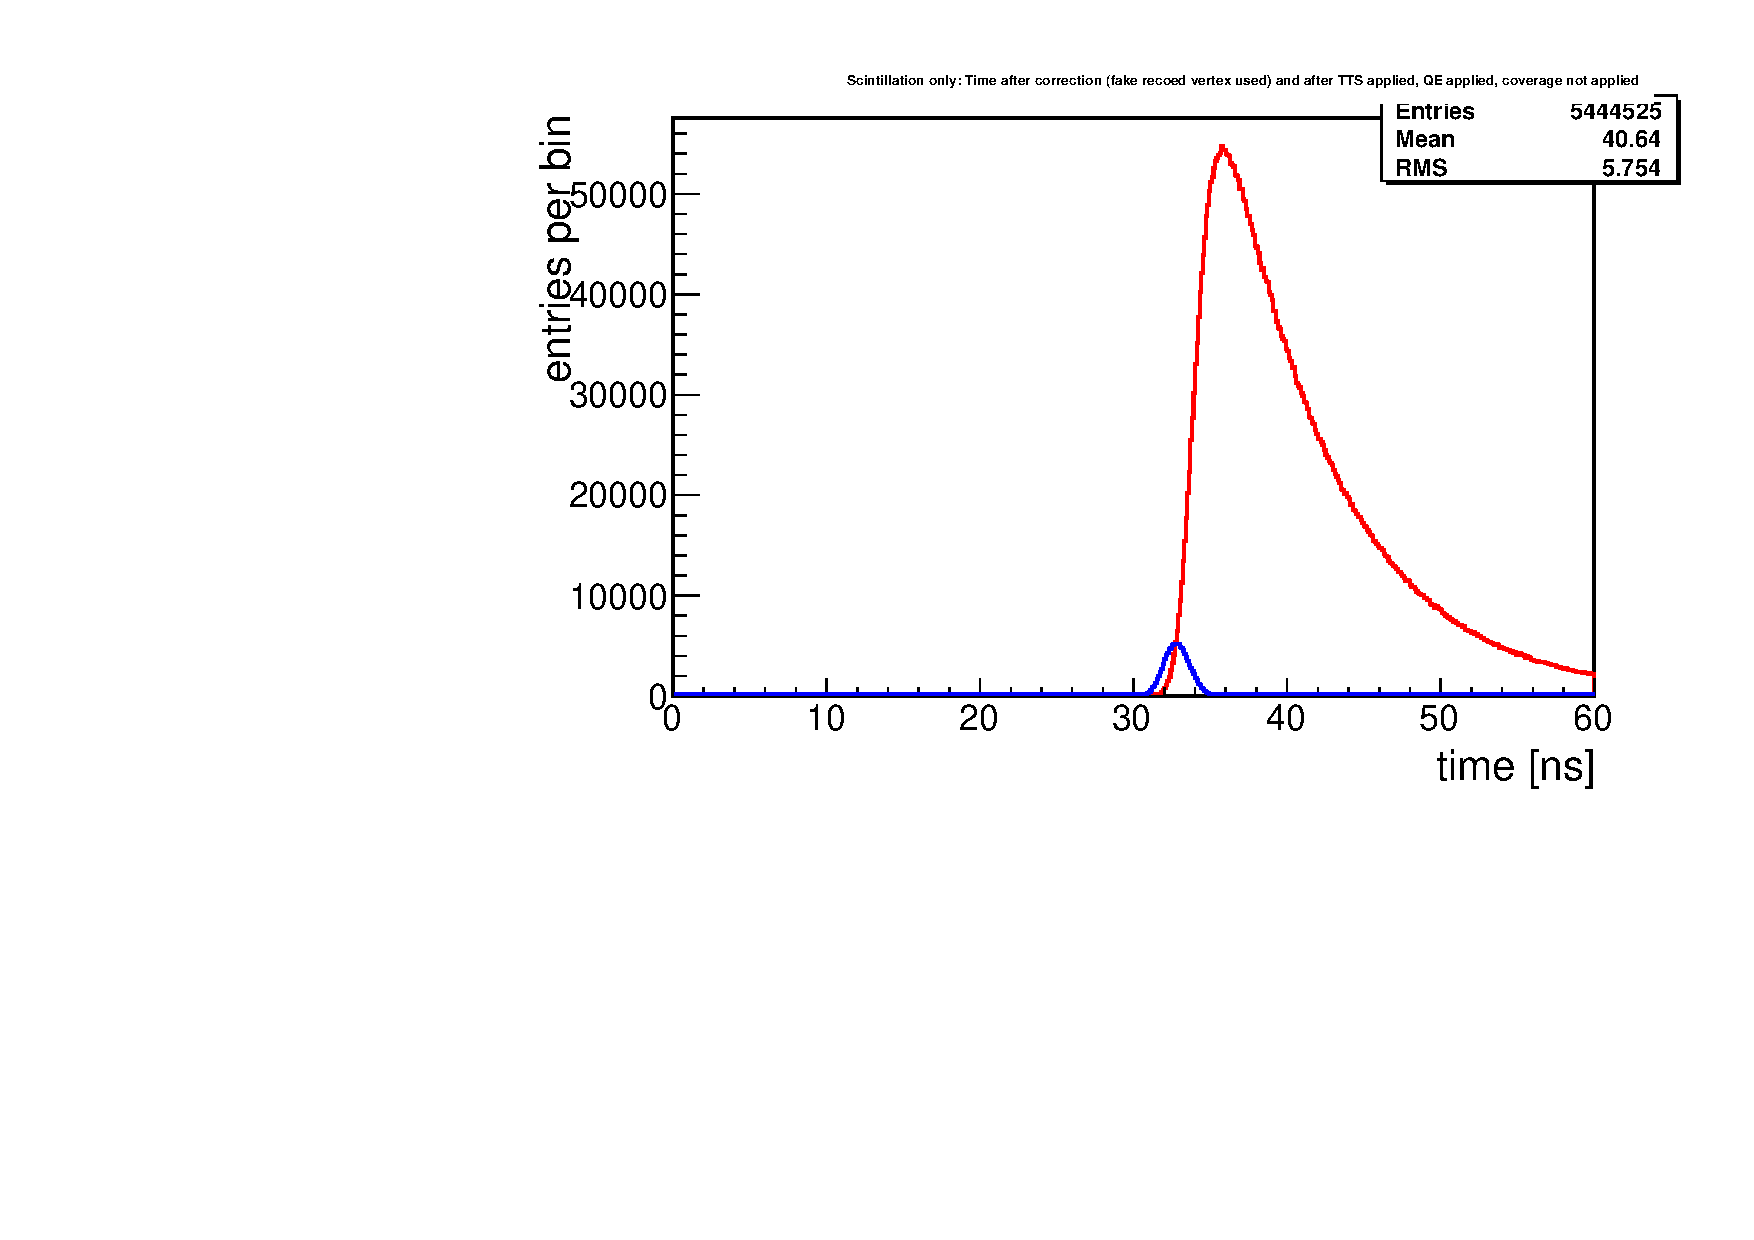
\includegraphics[scale=0.40]{graphs/6p5Meter_5MeVElectrons_Bialkali_KamlandScintSpec_TIME.pdf}
%%        \caption[]{PE times after TTS application for the simulation of 1000 electrons (5~MeV) with default settings: Detector diameter = 6.5~m, bialkali photocathode, KamLAND scintillator emission spectrum, TTS = 0.1~ns ($\sigma$). PEs from Cerenkov light (black) and scintillation light (red) are compared. The number of PEs per event after a 34.0~ns time cut is 171 from scintillation and 108 from Cerenkov. \label{6p5Meter_5MeVElectrons_Bialkali_KamlandScintSpec_TIME}}
%%        \end{center}
%%\end{figure}
%%\begin{figure}
%%        \begin{center}
%%        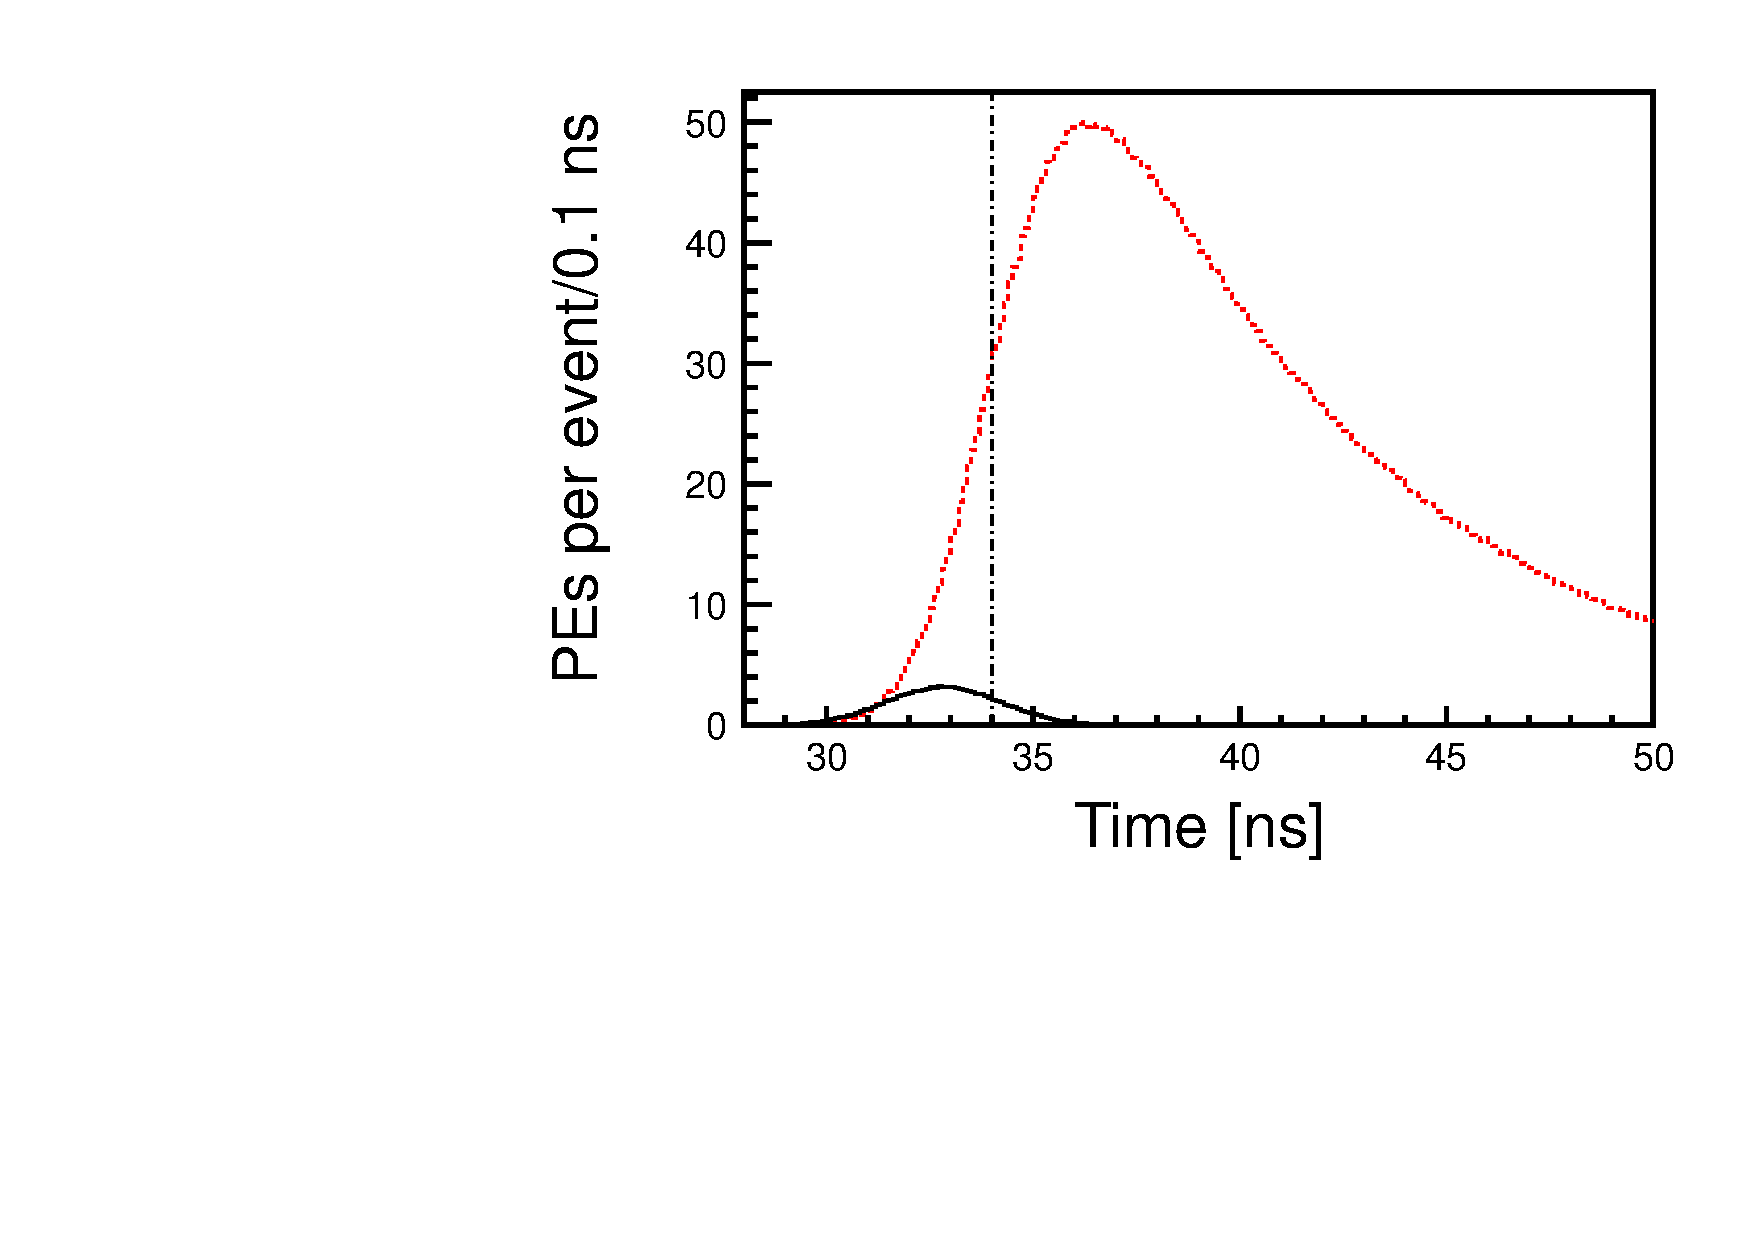
\includegraphics[scale=0.40]{graphs/6p5Meter_5MeVElectrons_Bialkali_KamlandScintSpec_1p28nsTTS_TIME.pdf}
%%        \caption[]{PE times after TTS application for the simulation of 1000 electrons (5~MeV) with TTS = 1.28~ns: Detector diameter = 6.5~m, bialkali photocathode, KamLAND scintillator emission spectrum, TTS = 1.28~ns ($\sigma$). PEs from Cerenkov light (black) and scintillation light (red) are compared. The number of PEs per event after a 34.0~ns time cut is 349 from scintillation and 88 from Cerenkov. \label{6p5Meter_5MeVElectrons_Bialkali_KamlandScintSpec_1p28nsTTS_TIME}}
%%        \end{center}
%%\end{figure}

First we discuss the default simulation settings which are described in the previous section. Figure \ref{time_plot_comparison} (a) shows the TTS-smeared photoelectron detection time for 1000 simulated electrons with 5~MeV energy in the center of the detector with initial momentum direction coinciding with the x-axis. The photoelectrons induced by Cerenkov light arrive earlier, as expected due to the instantaneous emission and the differences in the photon speed. There is however overlap with the PE time distribution coming from scintillation light. In order to compare simulations with different parameters to each other a fixed time cut $t \leq$ 34.0~ns (or 33.0~ns?) is applied (using the truth information of the electron starting time) instead of an event-by-event time reconstruction (see Section \ref{reconstruction_sec} for reconstruction results). For the default simulation case, the number of PEs per event coming from Cerenkov light after the 34.0~ns time cut (108) is 98~\% of the total number of PEs from Cerenkov light (110). For scintillation the number of PEs after the time cut (171) is only 3.2~\% of the total scintillation-induced PEs (5445).  
\begin{figure}[bt]
        \begin{center}
        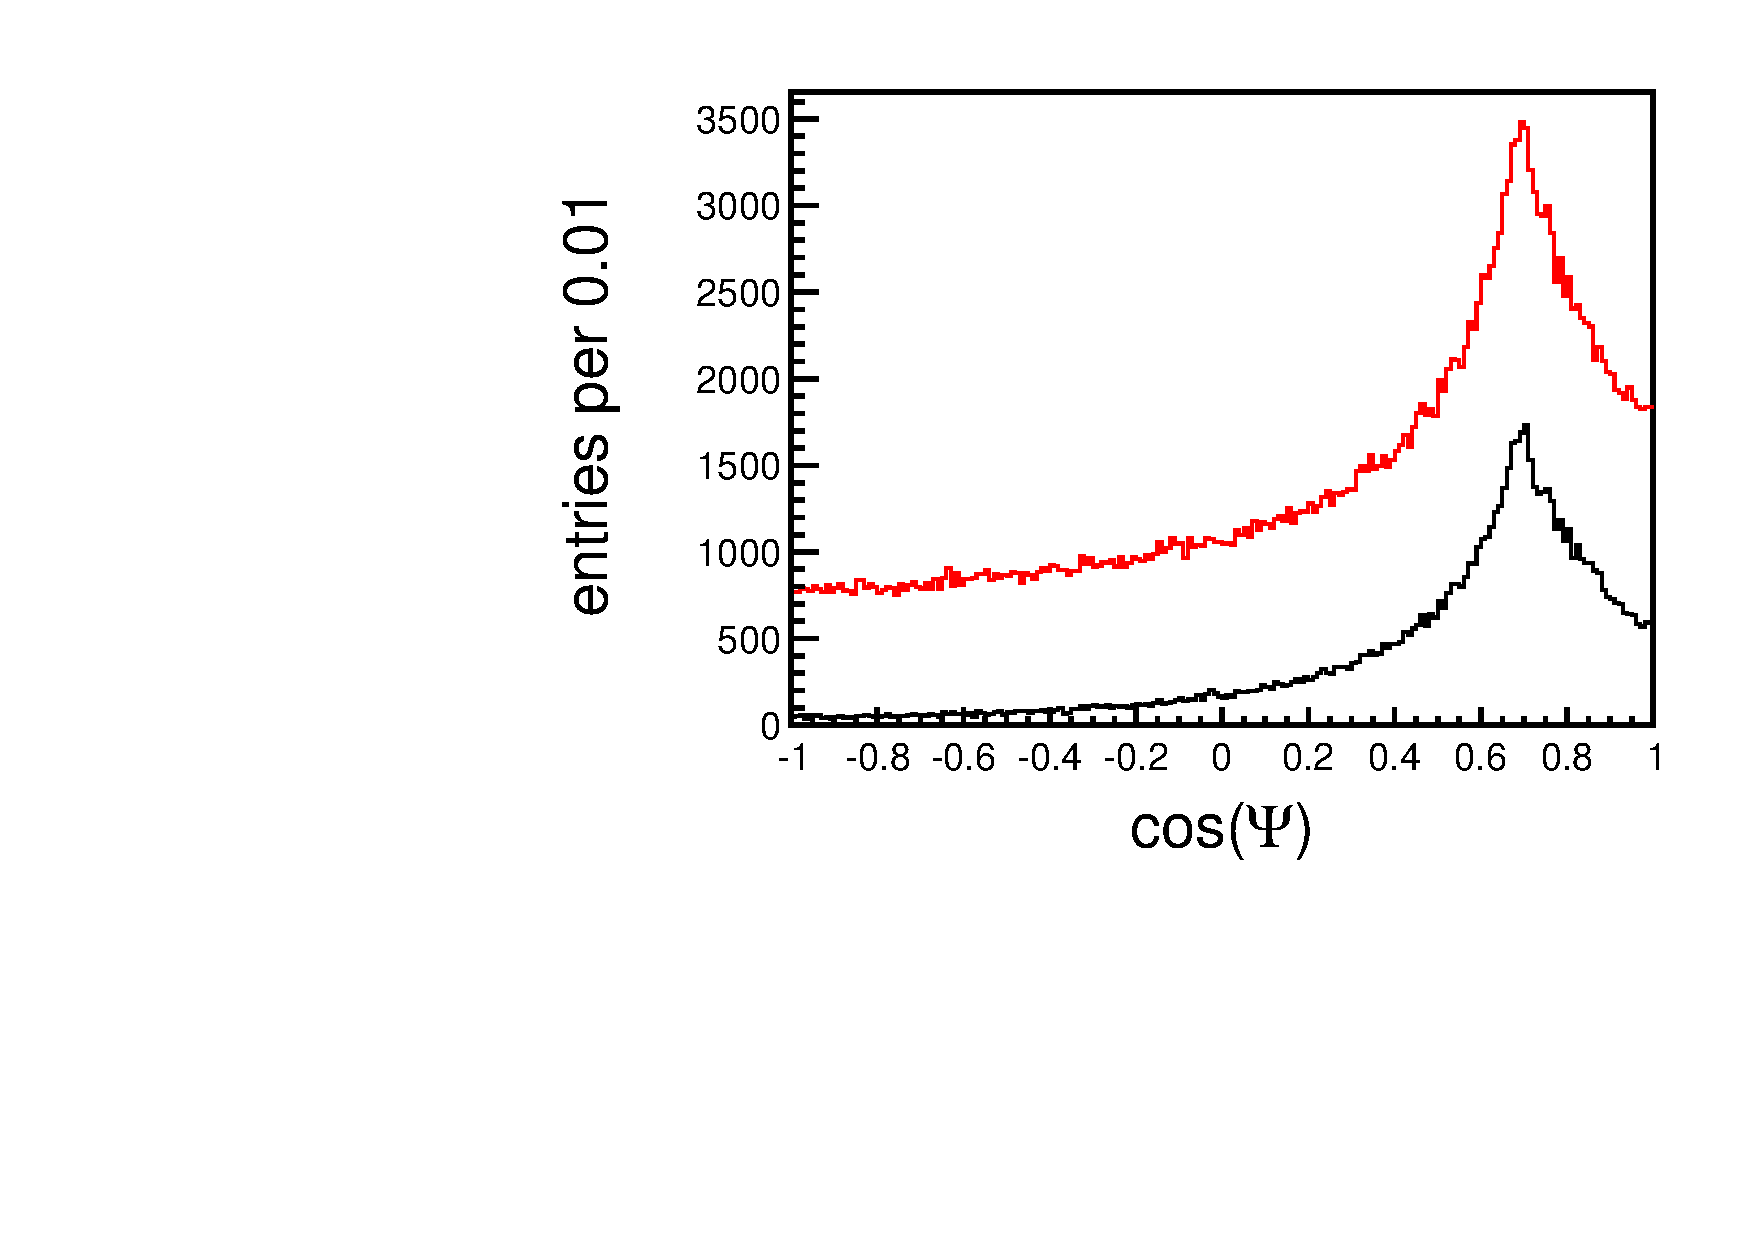
\includegraphics[scale=0.40]{graphs/cos_psi_comp_h.pdf}
        \caption[]{Angular distribution of photoelectron hits relative to the original electron direction for 1000 events (5~MeV electrons). Default simulation settings were used. A 33.0~ns time cut (black) is compared with a 34.0~ns time cut (red). \label{cerenkov_cone}}
        \end{center}
\end{figure}

Figure \ref{cerenkov_cone} displays the PE hit pattern after the 34.0~ns time cut has been applied (1000 events plotted together). Although this time cut is an oversimplification of actual time reconstruction effects, we can use it to indicate the spatial distribution of hits after timing information has been used to separate Cerenkov and scintillation light. The Cerenkov ring structure can be clearly seen (opening angle between 40\textdegree and 50\textdegree) which demonstrates that the directional signal conveyed by the Cerenkov photons is not erased by scattering of the initial 5~MeV electrons.  

If the 17 inch KamLAND PMTs \cite{tbd} (TTS = 1.28~ns) are used in the simulation, the broadening of the time distributions leads to a strongly decreased ratio of Cerenkov over Scintillation light after the time cut (see FIG. \ref{time_plots_comparison} (b)). This demonstrates that low photodetector TTS is critical for directionality reconstruction and motivates use of novel detector types.  

\section{Detector Wavelength Response}
\label{detector_wavelength_response_sec} 
Comlementary to lowering the photodetector TTS, optimization of the wavelength-dependent QE is promising. Since Cerenkov photons which passed 6.5~m of scintillator have higher average wavelengths than scintillation photons, a photodetector which is more sensitive at high wavelengths increases not only the absolute number of PEs but also the ratio between Cerenkov- and scintillation-induced PEs. Therefore, a simulation has been run with the QE of an extended red-sensitive GaAsP photocathode (digitized Hamamatsu R3809U-63 QE data was used).
%%\begin{figure}
%%        \begin{center}
%%        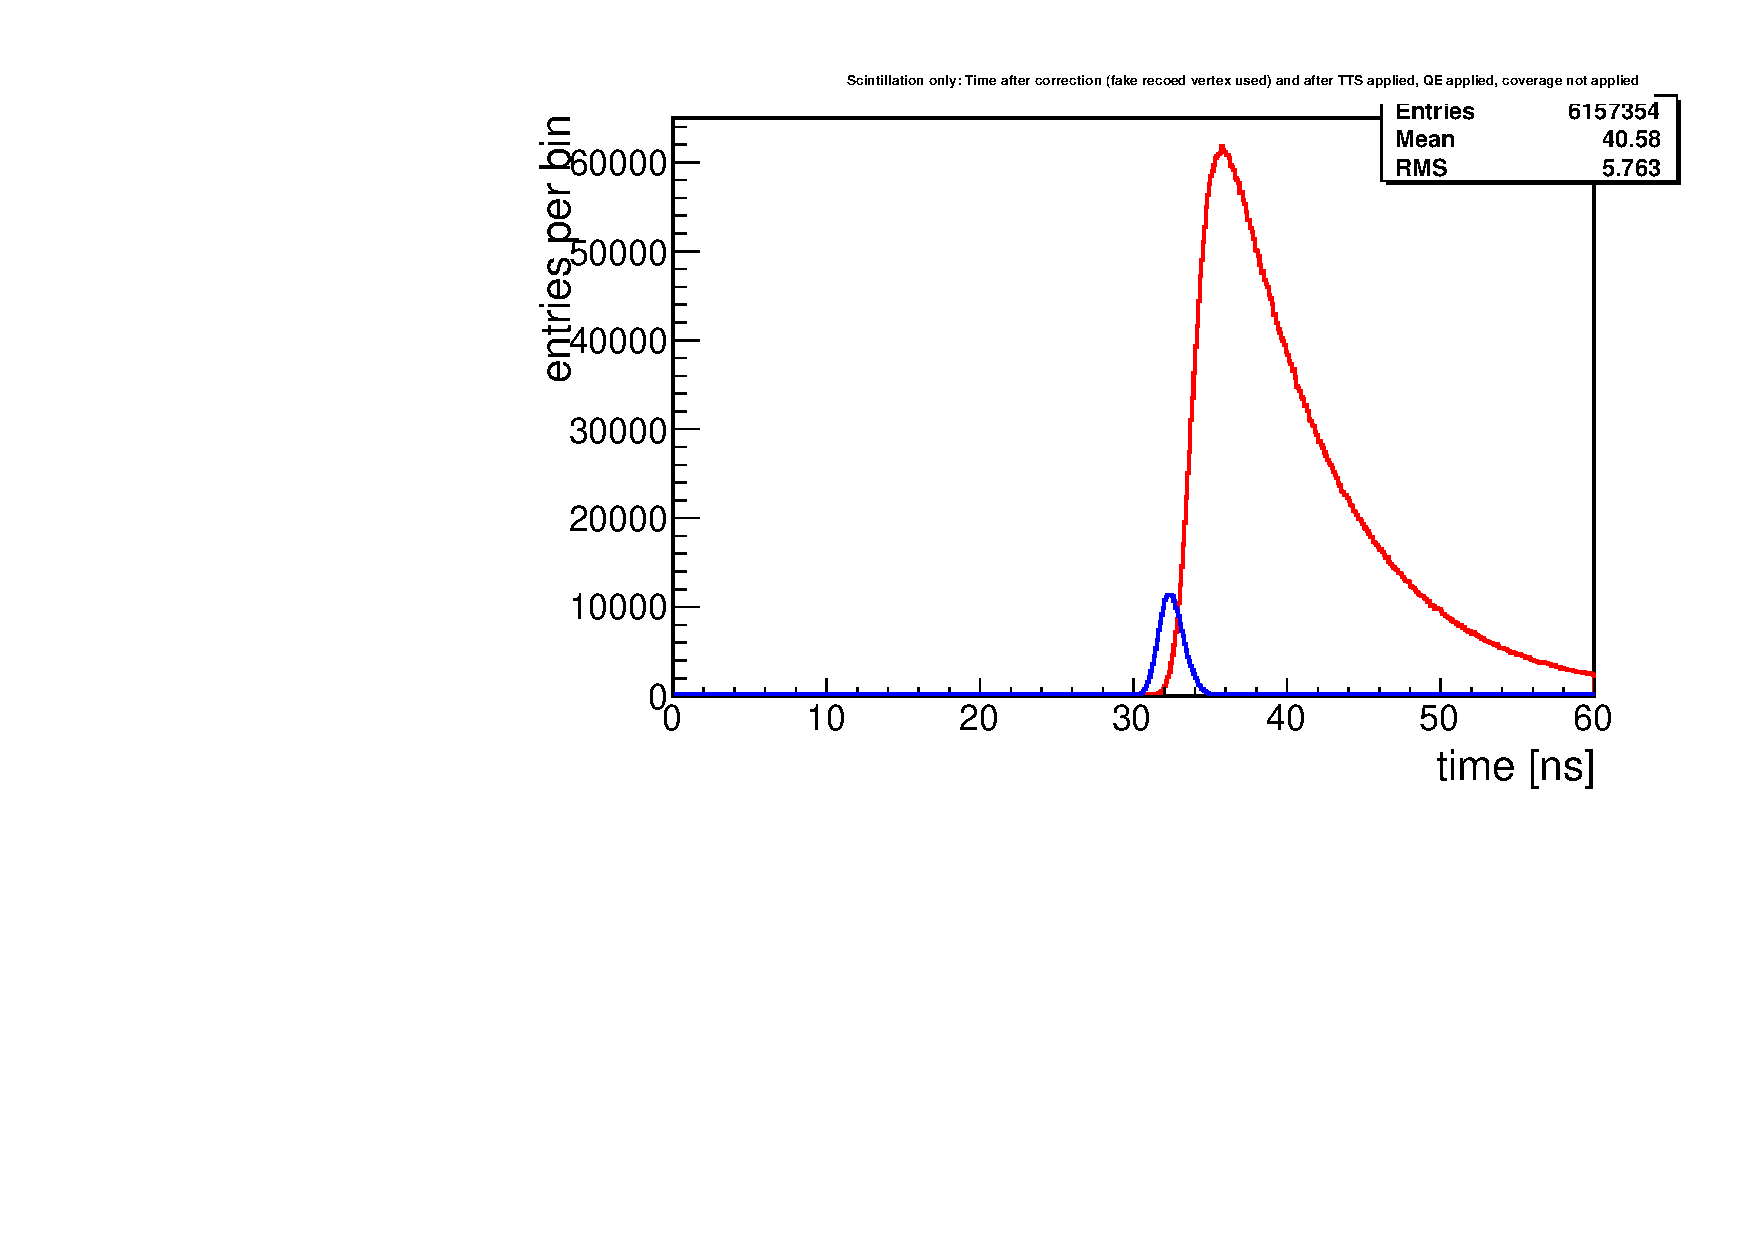
\includegraphics[scale=0.40]{graphs/6p5Meter_5MeVElectrons_RedSensitiveQE_KamlandScintSpec_TIME.pdf}
%%        \caption[]{Effectively reconstructed PE times for the simulation of 1000 electrons (5~MeV) with red-sensitive photocathode: Detector diameter = 6.5~m, red-sensitive GaAsP photocathode, KamLAND scintillator emission spectrum, TTS = 0.1~ns ($\sigma$). PEs from Cerenkov light (black) and scintillation light (red) are compared. The number of PEs per event after a 34.0~ns time cut is 50.8 from scintillation and 171 from Cerenkov. \label{6p5Meter_5MeVElectrons_RedSensitiveQE_KamlandScintSpec_TIME}}
%%        \end{center}
%%\end{figure}
Figure \ref{time_plots_comparison} (c) shows the results for the modified simulation with high QE in the red spectral region. The higher absolute number of PE coming from Cerenkov light (factor of $\approx$ 2) and the increased Cerenkov/scintillation ratio (factor of $\approx$ 1.6) after the time cut would significantly enhance the directionality reconstruction capabilities.  

\section{Scintillator Emission Spectrum}
\label{scintillator_emission_sec}
One important contributing factor to the separation in time between Cerenkov and scintillation photon hits is the higher average light speed for the photons coming from the Cerenkov effect due to their higher average wavelength. In this section we present two more sets of simulations where the scintillator emission spectrum was changed. 

Recently, the use of quantum dots (QDs) in liquid scintillators has been studied as a possibility to improve future large scale neutrino experiments \cite{tbd}. One important motivation is the control of the emission spectra by tuning the size or composition of the quantum dots. The emission spectrum of alloyed core/shell CdS$_x$Se$_{1-x}$/ZnS Trilite450 \cite{tbd} quantum dots was measured. This spectrum is a symmetric peak centered around 461~nm with FWHM = 29~nm. 

%%\begin{figure}
%%        \begin{center}
%%        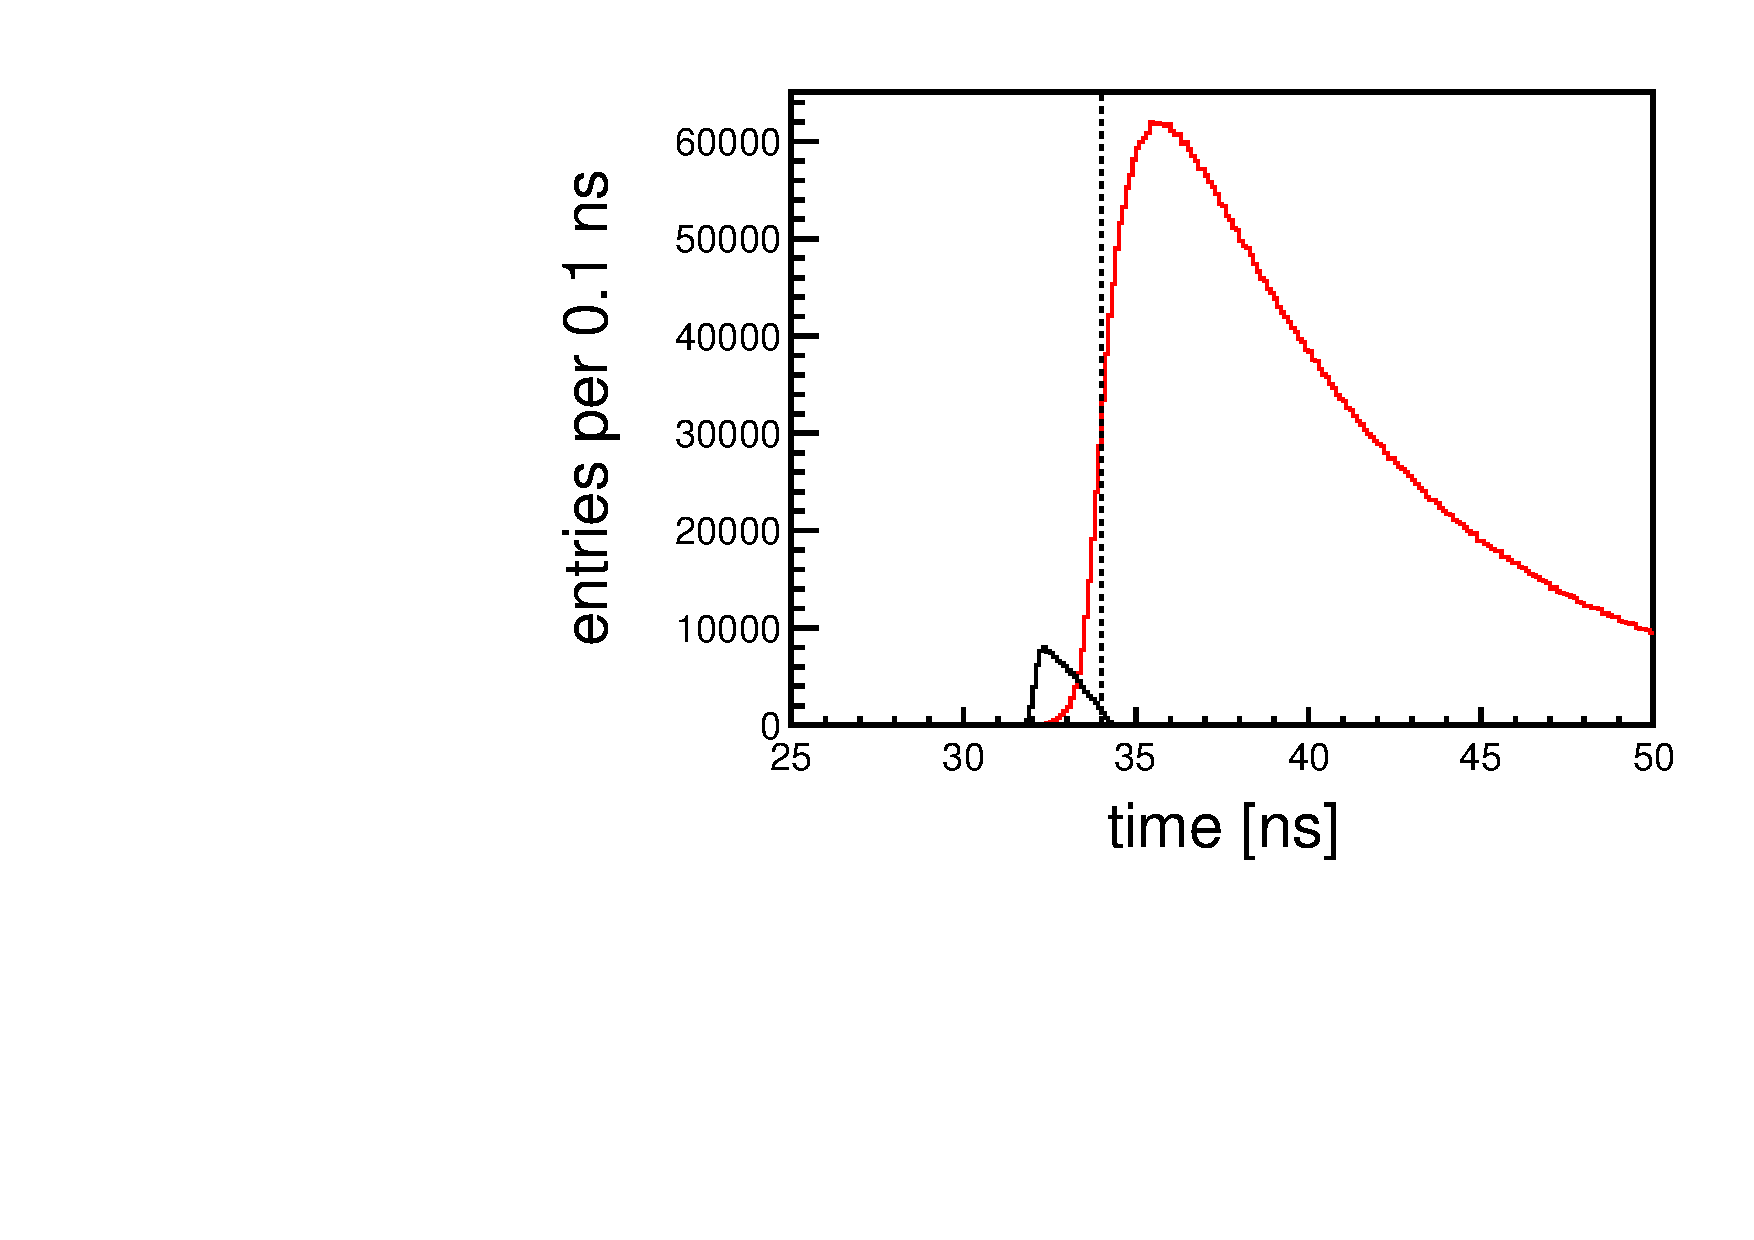
\includegraphics[scale=0.40]{graphs/6p5Meter_5MeVElectrons_Bialkali_QD384nmScintSpec_TIME.pdf}
%%        \caption[]{PE times for the simulation of 1000 electrons (5~MeV) with a quantum dot emission spectrum centered at 384~nm: Detector diameter = 6.5~m, bialkali photocathode, QD emission spectrum at 384~nm, TTS = 0.1~ns ($\sigma$). PEs from Cerenkov light only (black) and scintillation light only (red) are compared. The number of PEs per event after a 34.0~ns time cut is 124 from scintillation and 107 from Cerenkov. \label{6p5Meter_5MeVElectrons_Bialkali_QD384nmScintSpec_TIME}}
%%        \end{center}
%%\end{figure}  

In order to isolate the effect of a different emission spectrum, the other simulation settings, including the KamLAND absorption spectrum are kept unchanged. Compared to the default case shown in FIG. \ref{time_plot_comparison} (a) the separation is worse because the scintillation light wavelengths are higher than in the KamLAND emission spectrum. However, advances in the production of commercial quantum dot samples could yield quantum dots which have similar, single peak emission shapes at lower wavelengths. This case has been simulated using the same spectral shape of the measured Trilite450 emission but shifted to lower wavelengths such that the emission peak is centered at 384~nm. This peak emission value has been measured for other types of QDs, however with a much more pronounced tail \cite{tbd}. The resulting PE time distribution shows a slightly clearer separation of Cerenkov and Scintillation light. After the 34.0~ns cut on the TTS-smeared PE time we obtain a higher Cerenkov/scintillation ratio compared to the default simulation: The number of Cerenkov-induced PE after the time cut is unchanged while the number of PEs coming from scintillation light is decreased due to the higher average photon travel times.  

\section{Energy Dependence and Detector Size}
\label{edep_size_sec}
include this? 

The number of Cerenkov photons decreases disproportionally with decreasing electron energy. The number of PEs after the 34.0~ns time cut for 1~MeV electrons is 37 PE from scintillation and 13 PE from Cerenkov light. This illustrates that directionality reconstruction benefits from higher initial energies but even at 1~MeV there might be accessible directionality information.  

An additional set of simulations of a 0.65~m diameter ($\approx$ 1~m$^3$) detector with otherwise default parameters was performed. In the smaller detector the chromatic dispersion is not as important and absorption in the scintillator bulk is reduced. The latter effect increases the absolute number of photoelectrons. The former effect, on one hand, reduces the separation in time between Cerenkov and Scintillation light. On the other hand, it reduces the broadening of both time distributions which helps more sophisticated vertex and track reconstruction with the help of fast photodetectors like for example the LAPPDs. 

%tbd (calculate numbers): However, with the simplified effective vertex reconstruction and a time cut of 3.4~ns we get  PEs from scintillation and 87 PEs from Cerenkov. The time cut was adjusted such that the fraction of selected PEs from Cerenkov light matches the fraction in the large detector ($\approx$ 58\%). The QD spectrum discussed in section \ref{scintillator_emission_sec} (both shifted and unshifted) did not change the PE time distribution significantly. We also simulated the red-sensitive photocathode discussed in section \ref{detector_wavelength_response_sec} in the small detector. The amount of PE increases again significantly and with the 3.265~ns time cut the number of PE coming from Cerenkov light is 182 while the number of PE from scintillation light is 96. 

In summary, the photodetector properties (TTS and QE) become more important relative to the scintillator emission and absorption spectra when the detector size is decreased from 6.5~m to 0.65~m.


%%idea: use (some) PMTs with high QE for high lambda (and/or low QE for normal lambda). 
%% add some more info why we are interested in a smaller detector
%% motivation: Daedalus/ISODAR (?), 0nuBB 
\section{Reconstruction}
\label{reconstruction_sec}
WCSimAnalysis is a Water Cherenkov reconstruction package developed by Andrew Blake for the Long Baseline Neutrino Experiment (LBNE collaboration). It provides a framework for generic event cleaning, track reconstruction, and particle id, and it comes equipped with variety of pre-built algorithms. A collaboration between Iowa State, the University of Chicago, and Argonne National Laboratory has continued adding to the code, developing new track-fitting techniques for Water Cherenkov detectors built around the unique capabilities of microchannel plate photodetectors (MCPs): timing resolutions below 100 picoseconds and imaging resolutions below a centimeter. In this paper, we use only the simple, low-level reconstruction tools native to the package, though in future works we hope to implement more sophisticated techniques.

The simplest approach to vertex reconstruction, used in this paper, is commonly referred to as a �point fit�. It assumes that, to first order, the light was emitted a single point in space-time (x0,y0,z0,t0). In reality, the light is emitted along the extended, multi-scattered track of the electron. However, at the energies discussed in this paper, the extent of the electron track is small (a few cm) compared to the scale of the detector, which has a radius of 6 meters. It is also small compared with the vertex resolutions typical of experiments with this scale. As starting point, the assumption works well. 

The first algorithm we use to find a seed vertex relies on exact numerical calculations of possible vertex candidates. Given a single point source, we need four constraints to solve for the four unknowns of the vertex. A collection of N random quadruplets of hits is selected and used to solve for N corresponding vertex candidates. Some of these solutions will produce nonsensical results due to optical scattering of the emitted light, slow decay constant of the scintillation, finite detector resolution, and the limitations of our assumption of a point source. Nonetheless, over the N unique quadruplets, we expect some of the solutions to lie near the true event vertex. In this paper we chose N to be 80, determined by trial and error. However, given many hundreds of hits, the number of possible 4-hit combinations is much larger and one can choose a different N to better suit one�s particular experimental context.

Once the 80 vertex candidates have been solved for, we test the goodness of each candidate and select the one that best fits the full ensemble of hits. Distances are calculated between each hit and the candidate point-source. From these distances, we calculate the transit time, given the speed of light in our scintillator medium. This transit time plus the t0 of the 4-vertex provides a predicted arrival time for each hit. The �time residual� is the calculated as difference between the predicted and the measured arrival time, given the vertex candidate. Since we assume a point-source in this paper, we use what we call the �simple time residual�, as distinct from the �extended time residual�, which assumes an extended, track-like geometry. The distribution of time residuals for each hit with respect to a vertex candidate has a width that is minimized when the hypothesis vertex is close to the true vertex. The t0 of the vertex candidate is left to float, and is adjusted to maximize the likelihood comparison with a Gaussian test function. The width of that gaussian test function is hand optimized to correspond with the width of the �best fit�. The vertex candidate with the largest maximum is selected to serve as the best candidate seed vertex. Once a single best seed vertex has been chosen, the same time-residual figure-of-merit is used in a MINUIT-based fit over a continuum of possible vertices in the neighborhood of the seed.

Once the vertex fitting is completed, we determine the direction by taking the centroid of all vectors pointing from the fitted event vertex and the hits on the detector. Since our initial time cut greatly enhances the purity of the Cherenkov light in this sample of hits and, since the Cherenkov light is directional (compared to the isotropic scintillation light), this fit provides a good measure of the track direction. This approach does not rely on the highly constrained Cherenkov geometry of the event, which contains further information. Future work will focus on better algorithms. Nonetheless, for a proof-of-principles, this method works sufficiently well..

\begin{figure}
        \begin{center}
        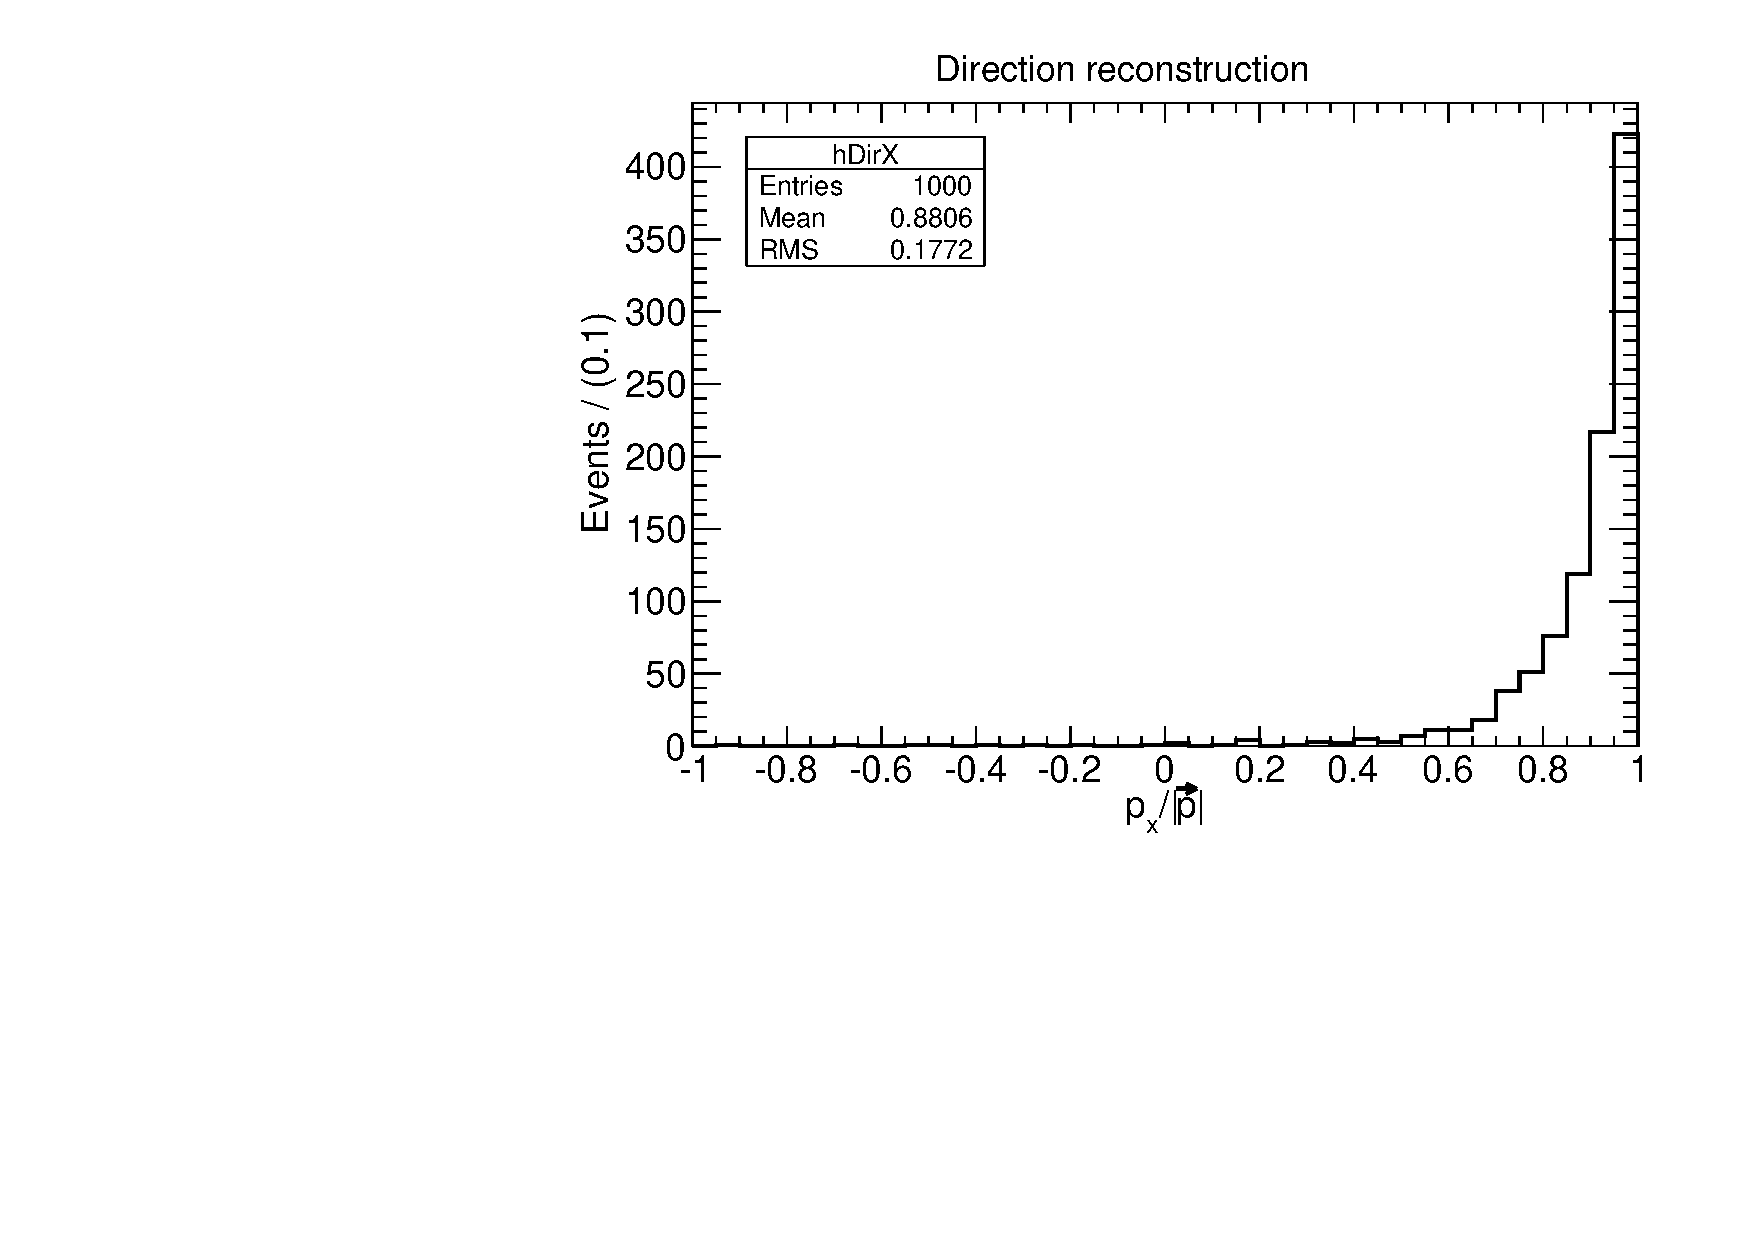
\includegraphics[scale=0.20]{graphs/hDirX.pdf}
        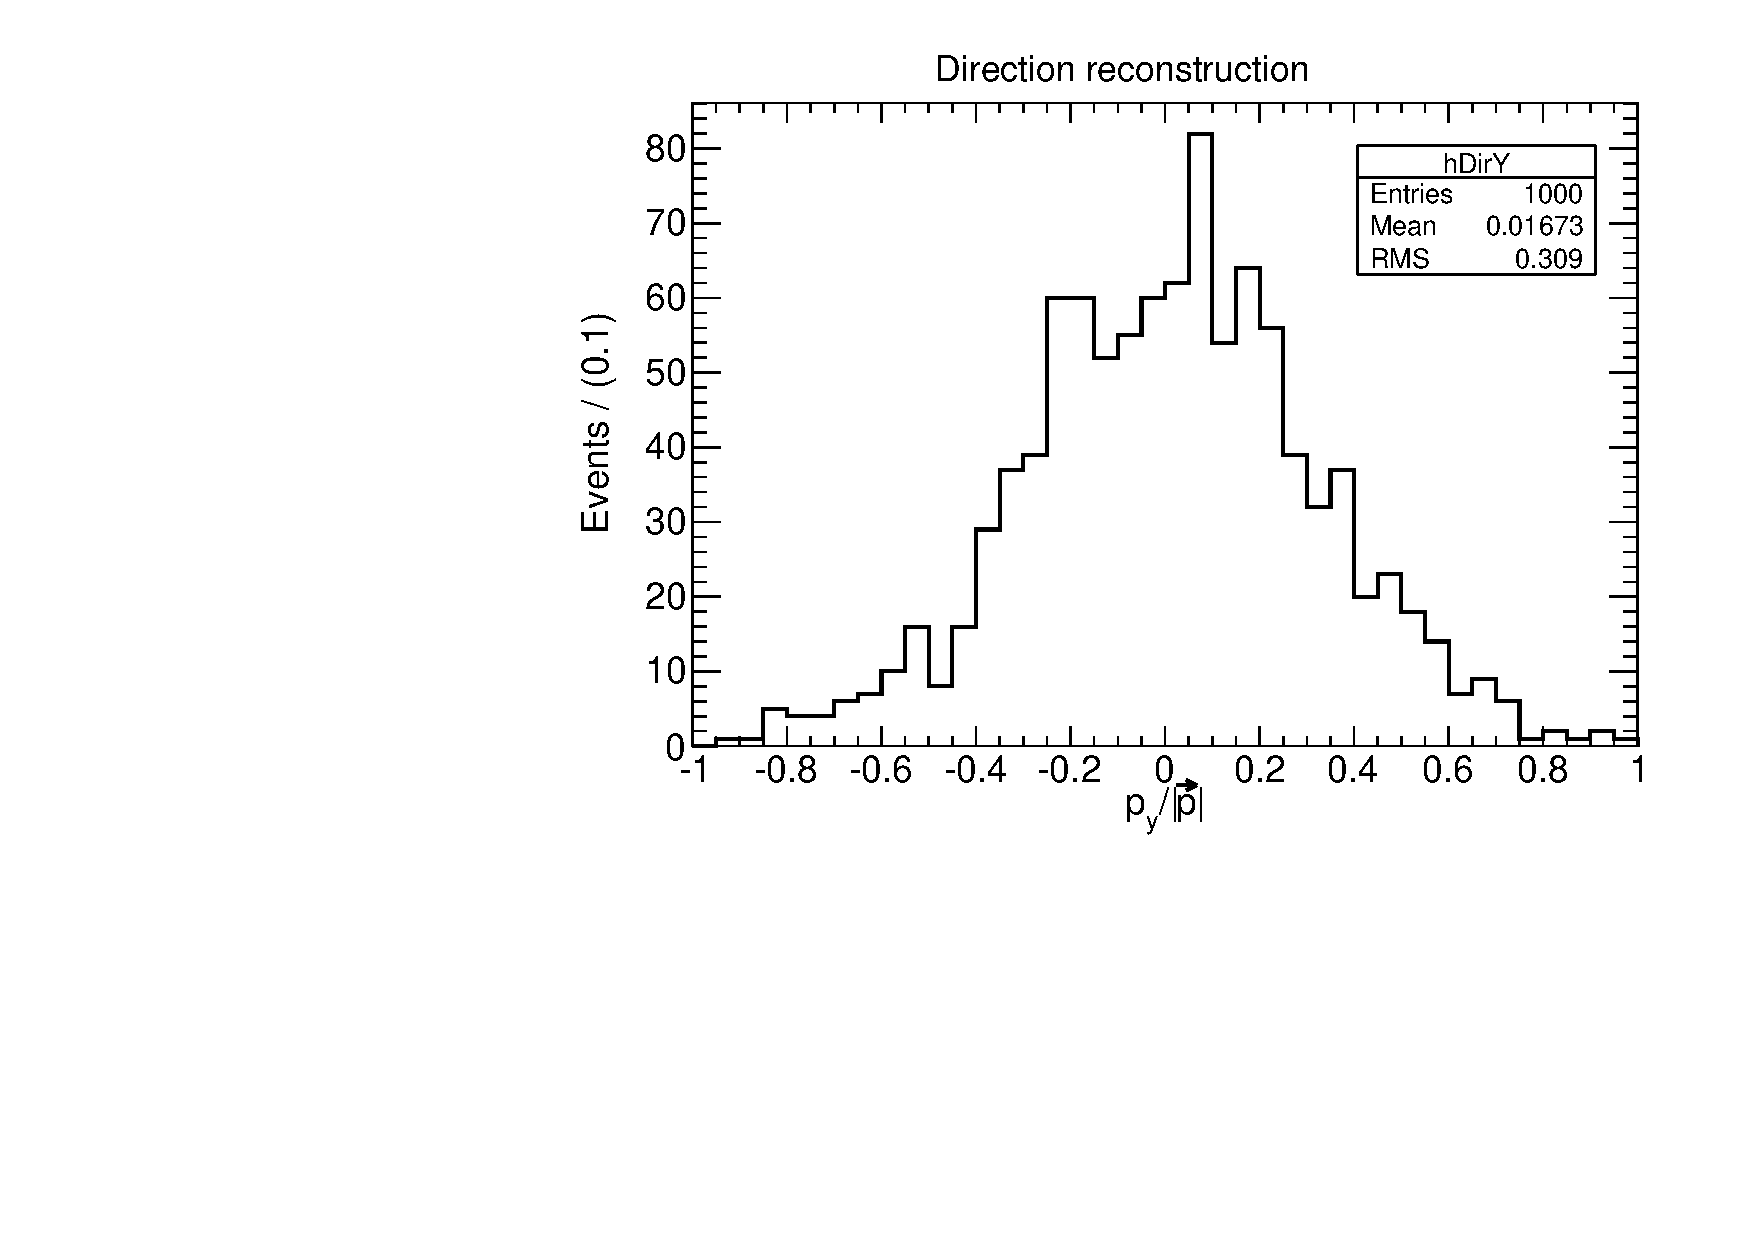
\includegraphics[scale=0.20]{graphs/hDirY.pdf}
        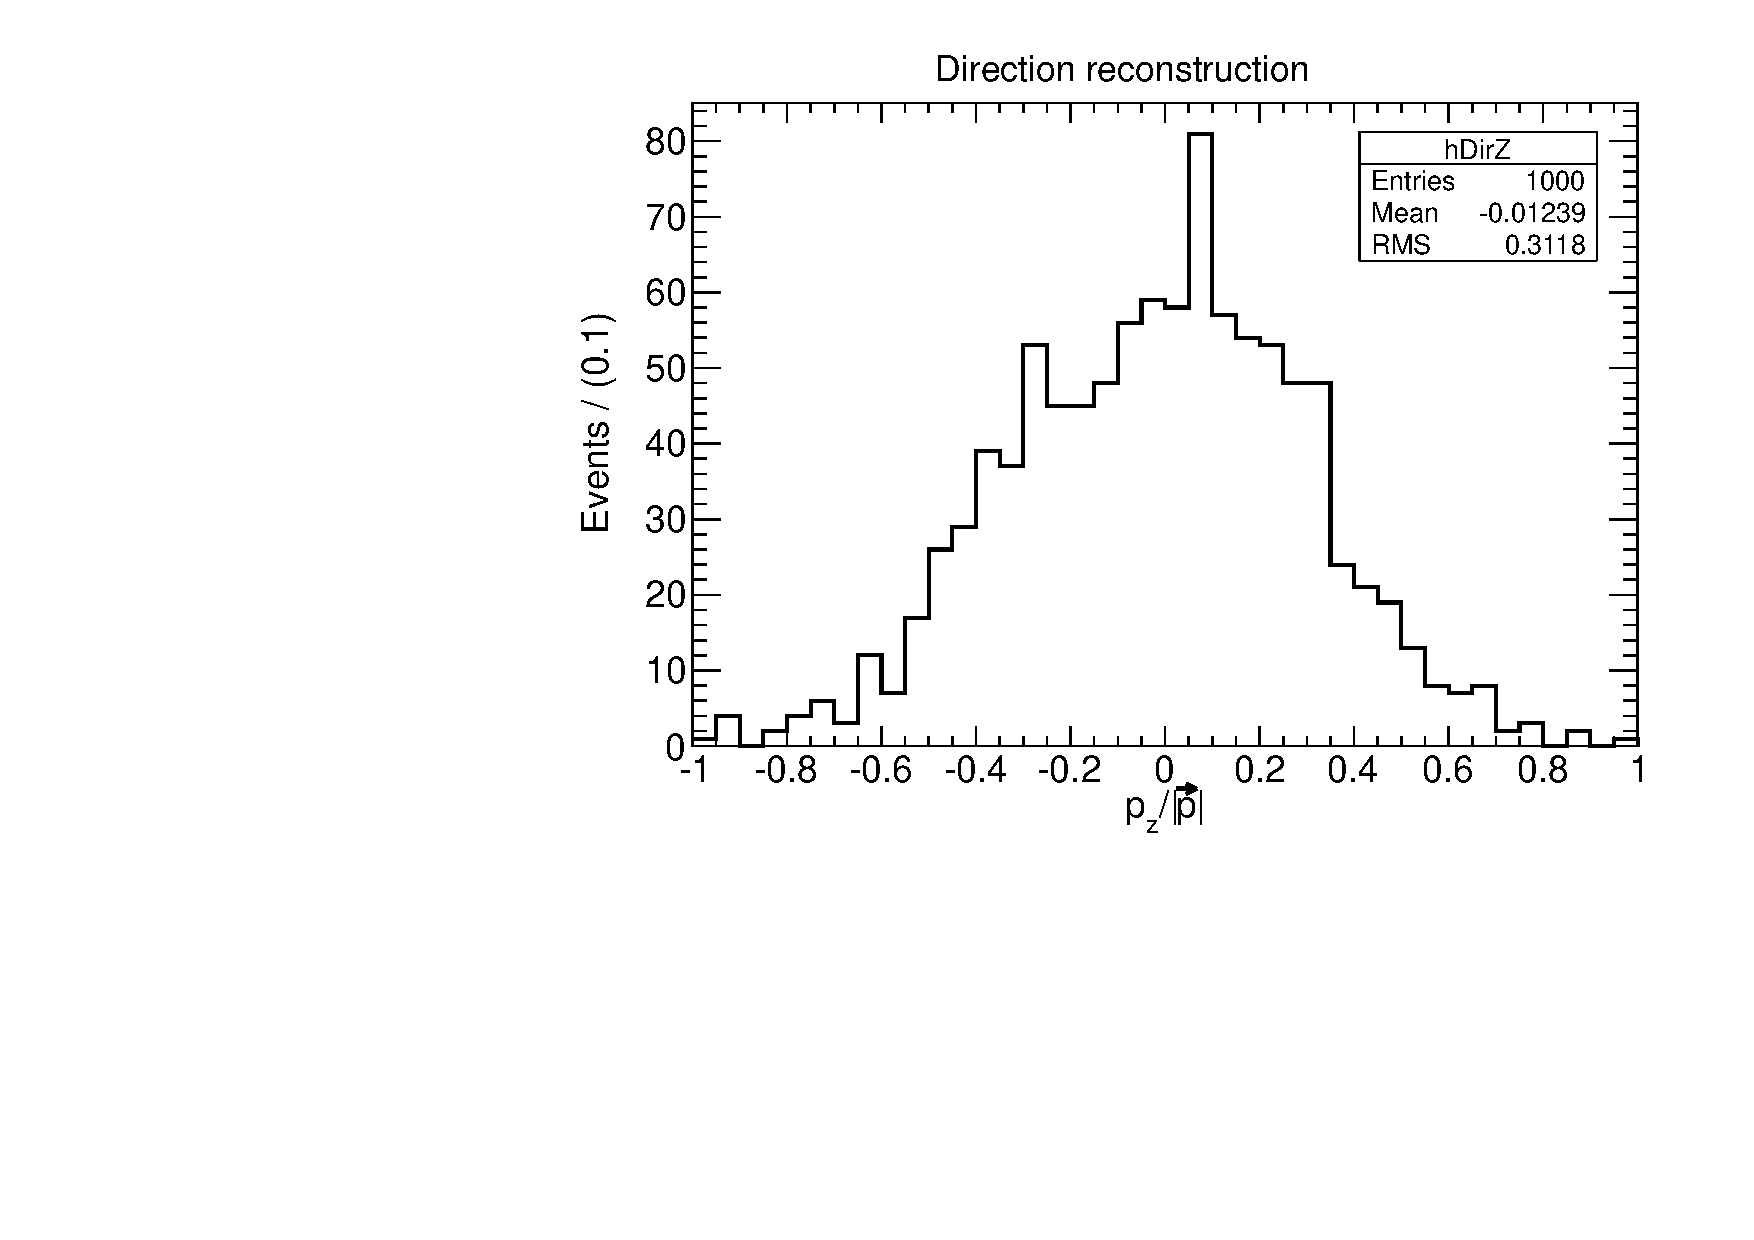
\includegraphics[scale=0.20]{graphs/hDirZ.pdf}	
         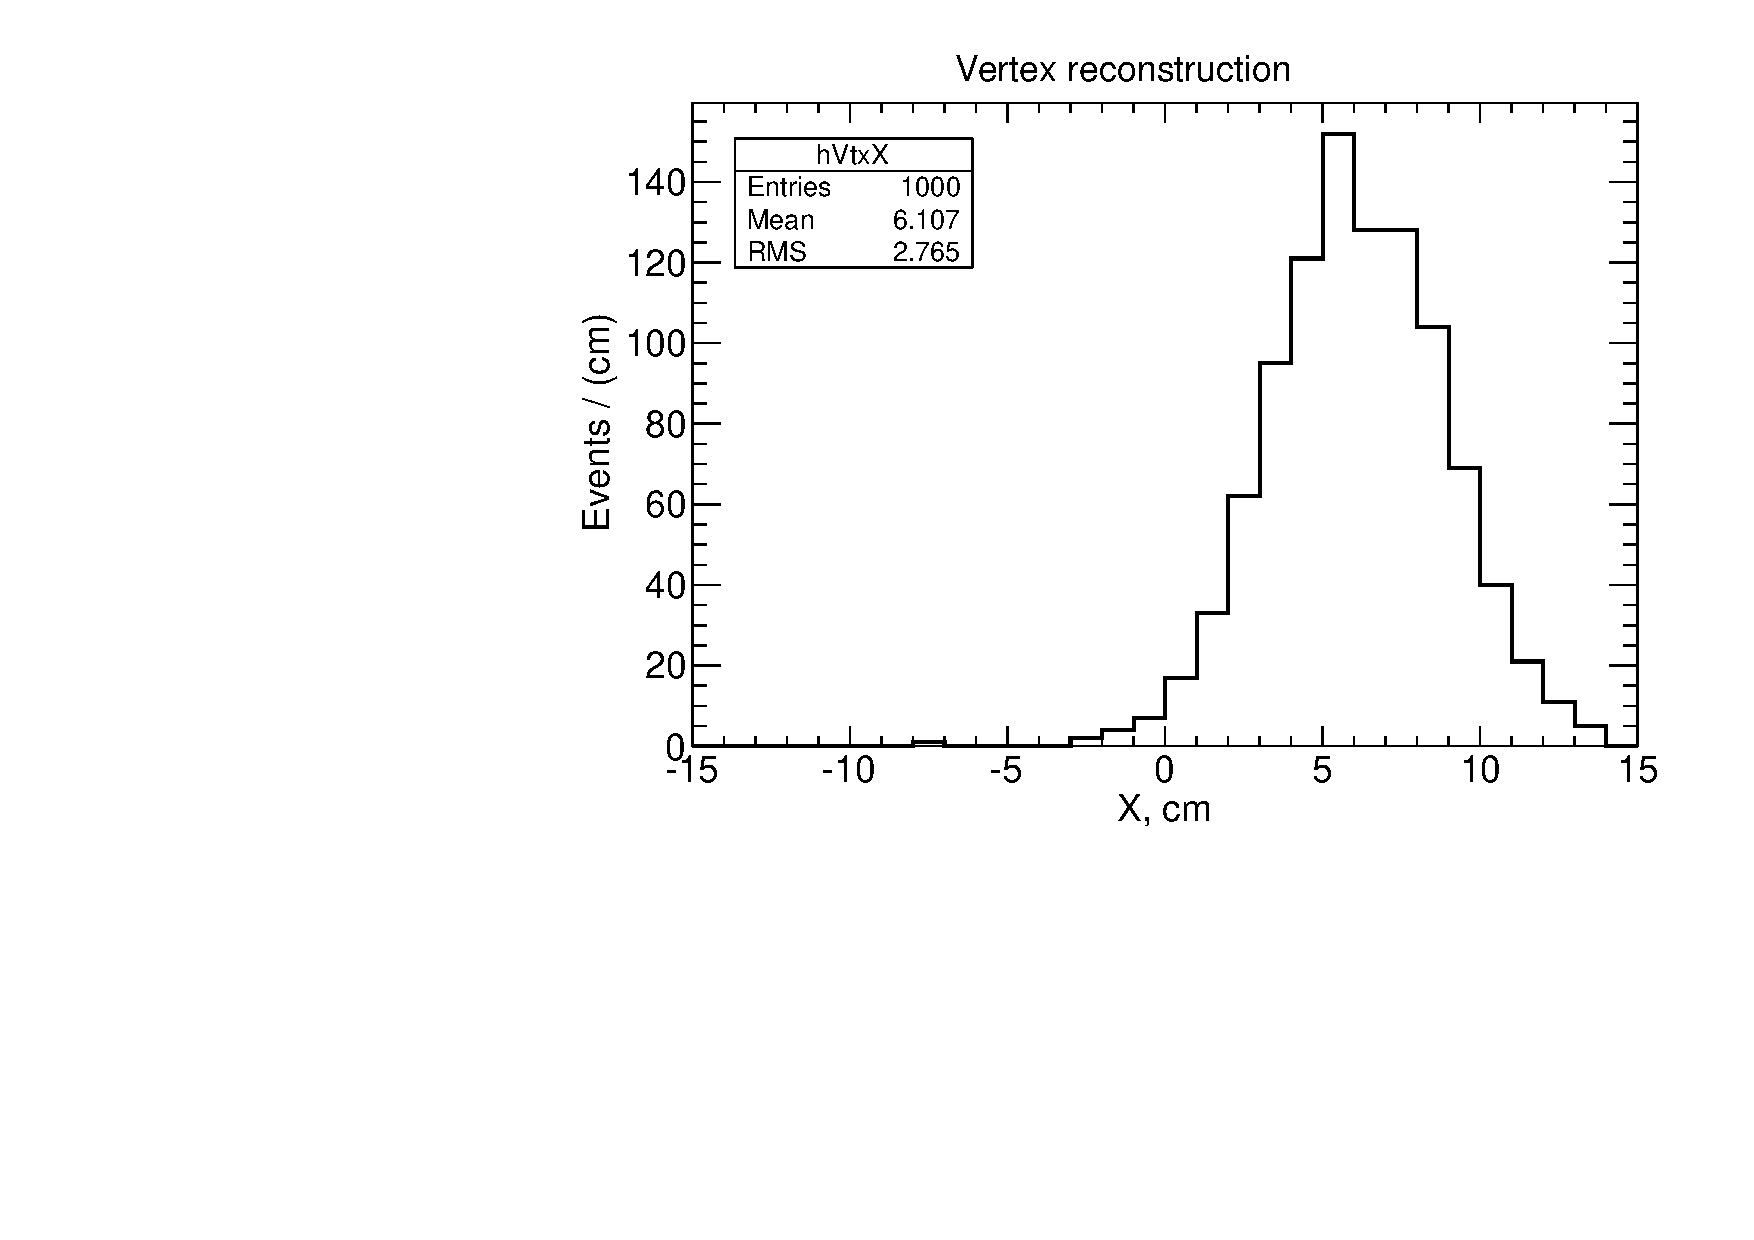
\includegraphics[scale=0.20]{graphs/hVtxX.pdf}
        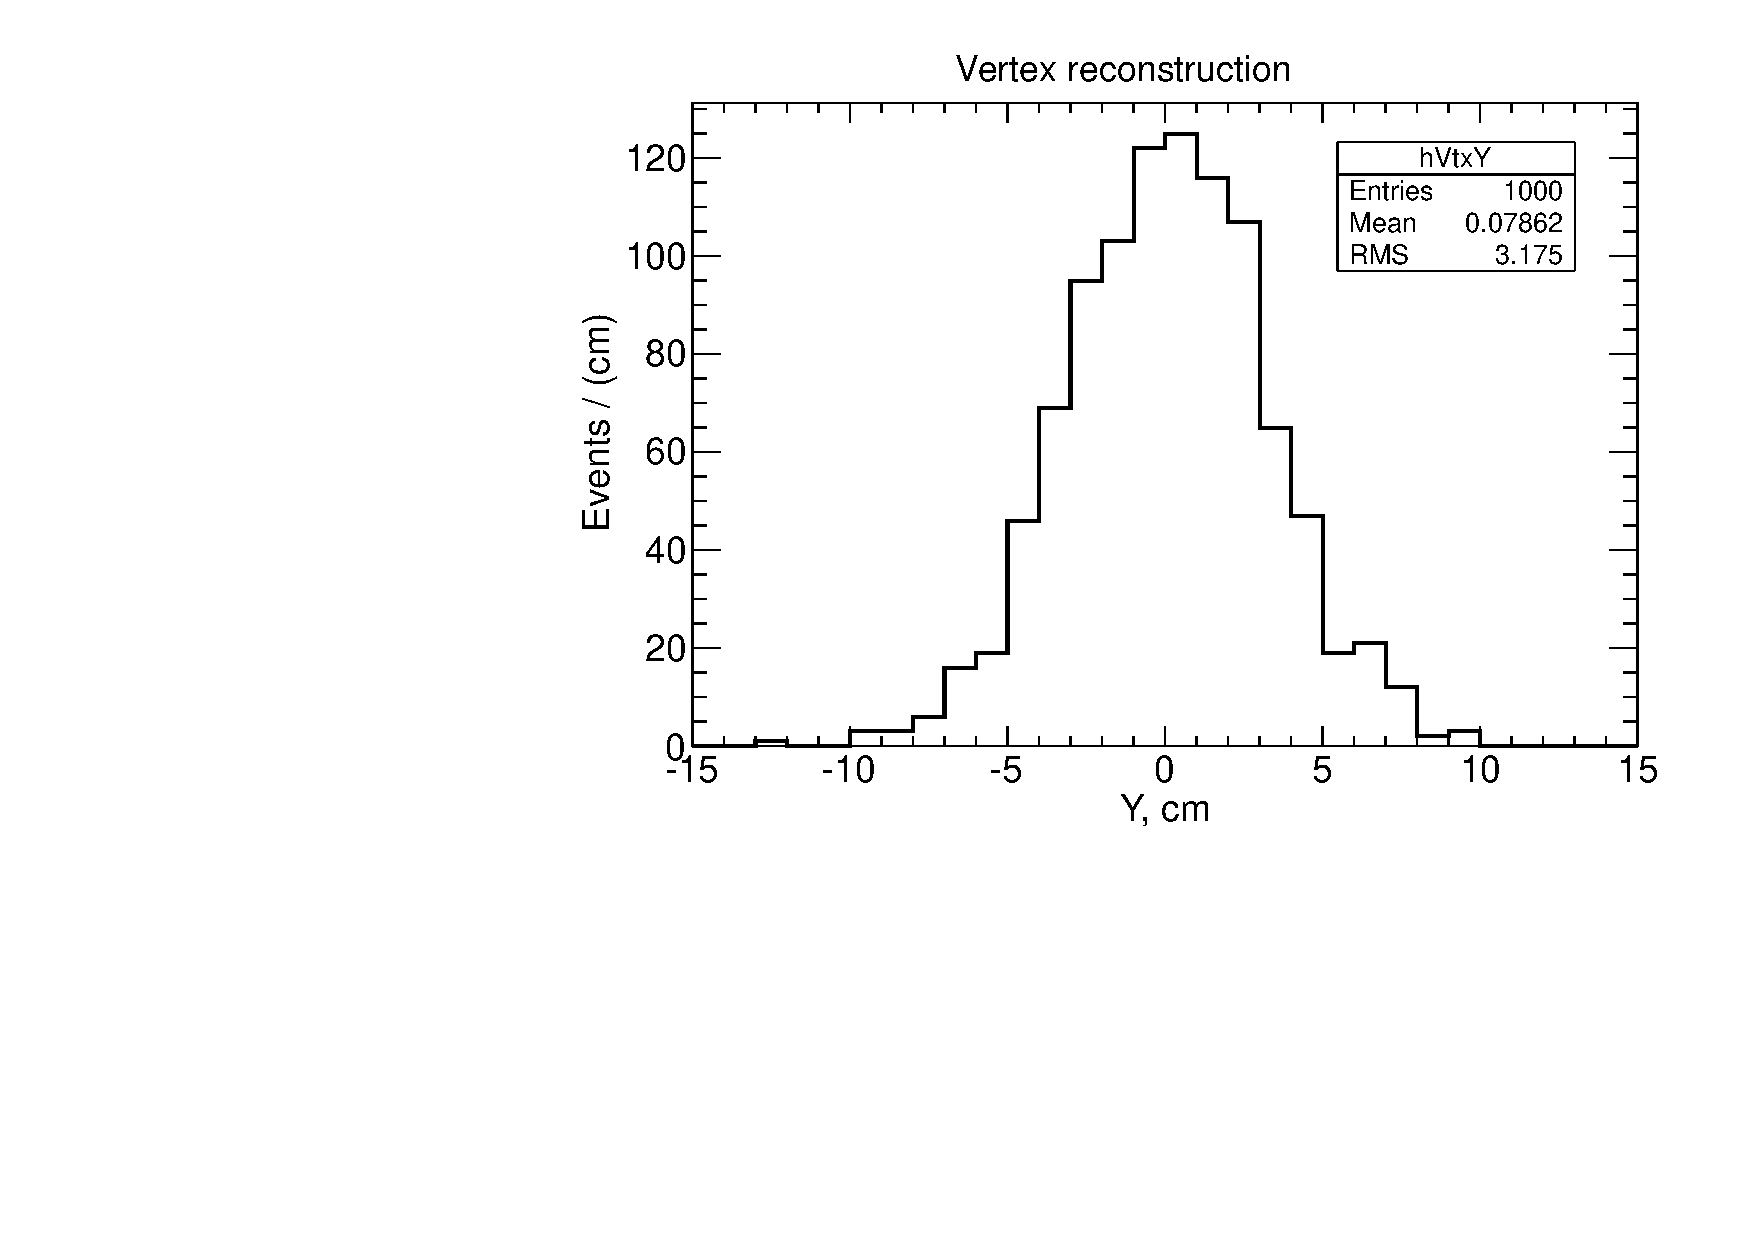
\includegraphics[scale=0.20]{graphs/hVtxY.pdf}
        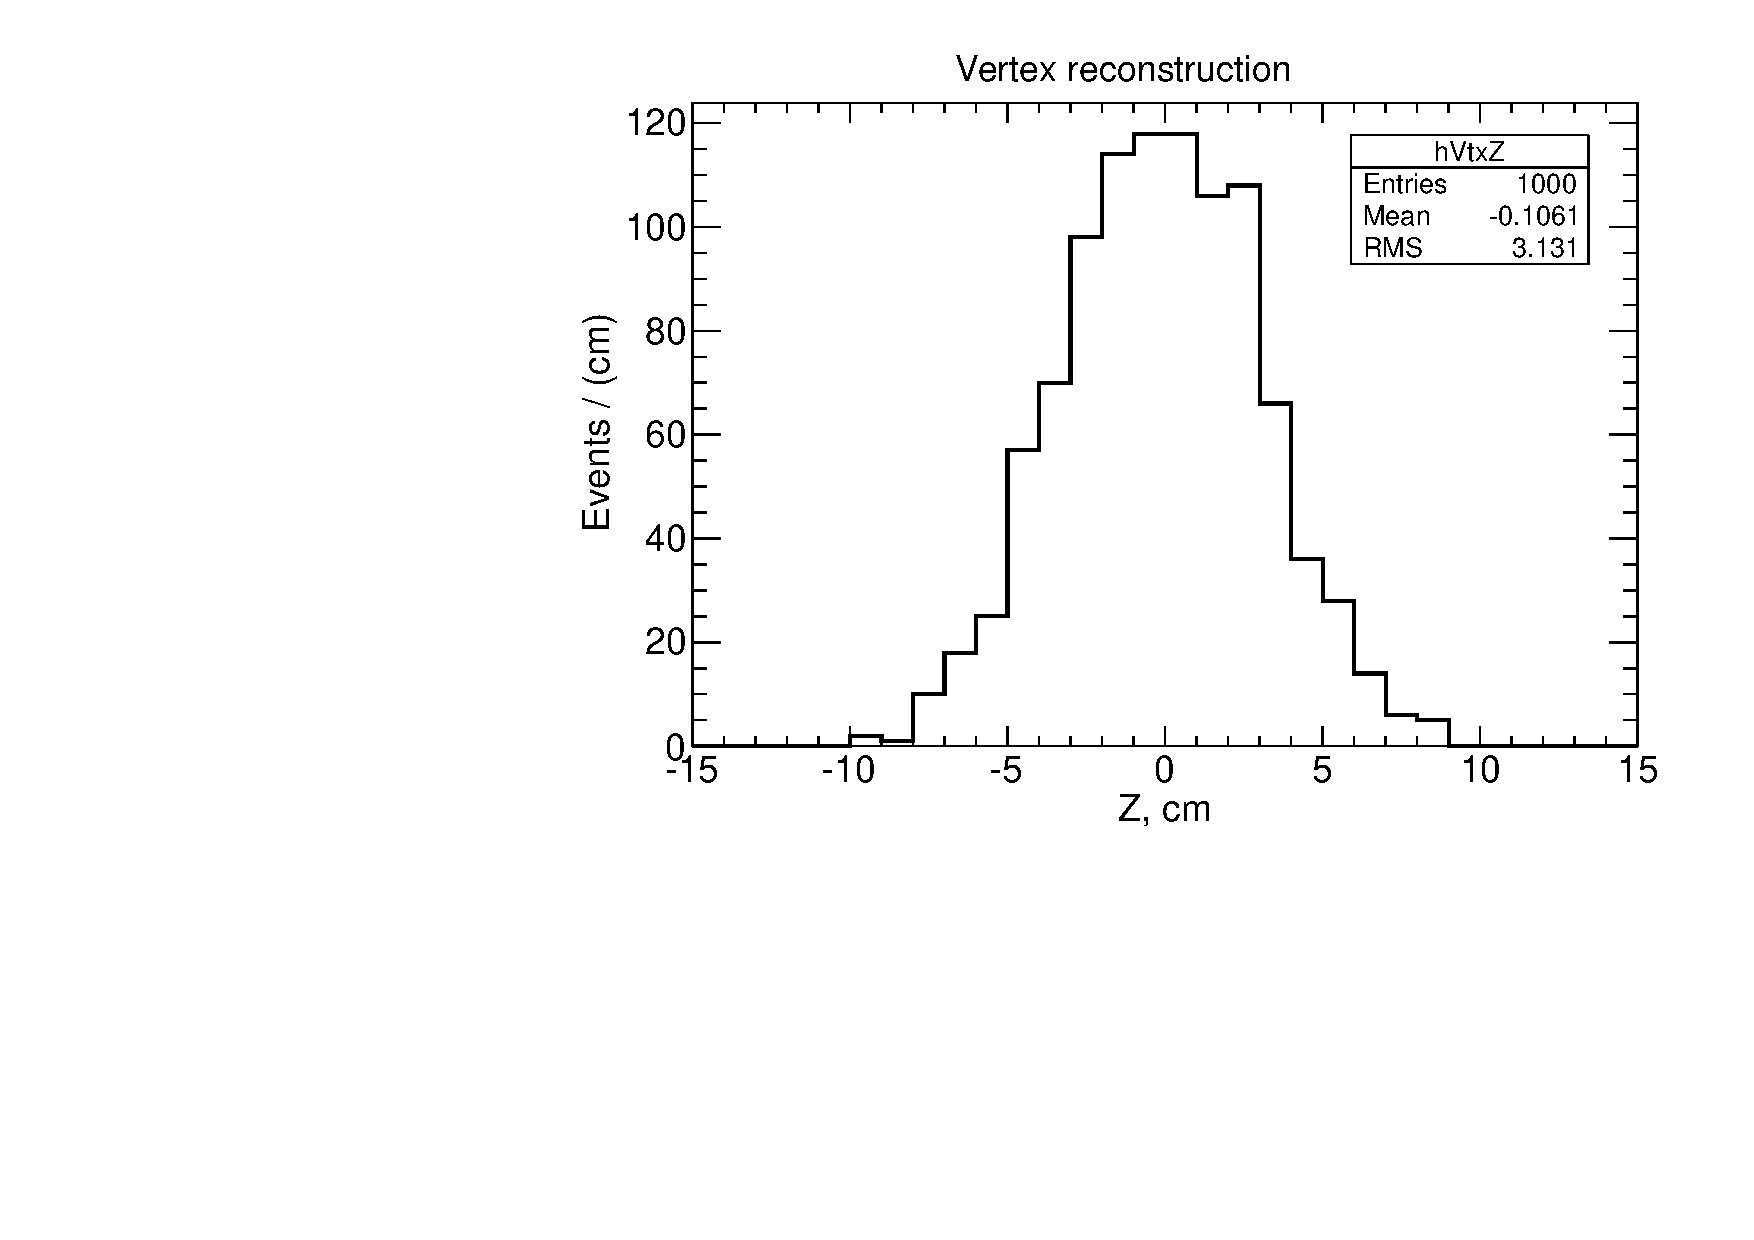
\includegraphics[scale=0.20]{graphs/hVtxZ.pdf}	
        \caption[]{ We need a caption.}
        \end{center}
\end{figure}  


\section{Conclusion}
This is going to work.

\section{Acknowledgements}
L. Winslow would like to thank for useful discussion on the topic. L. Winslow would also like to thank K. Arisaka for discussions on the possible reach of traditional PMTs and the characteristics of HPDs. A. Elagin, H.J. Frisch and M. Wetstein are supported by DOE XXXX. C. Aberle and L. Winslow are supported by funds from University of California Los Angeles.

\bibliography{DirectionBibliography}

%%20 inch PMTs: 
%%H.~Kume, S.~Sawaki, M.~Ito, K.~Arisaka, T.~Kajita, A.~Nishimura, and A.~Suzuki, Nucl. Instrum. Methods Phys. Res. \bf{205}, 443 (1983).
%%17 inch PMTs: 

\end{document}
